%Schriftart Format
\documentclass{article}
\usepackage[english]{babel}
\usepackage[utf8]{inputenc}
\usepackage[T1]{fontenc}
\usepackage{geometry}
\geometry{a4paper, portrait, margin=30mm, headsep= 32pt , headheight = 19pt, footskip = 40 pt}
\usepackage[]{placeins}
\usepackage{hyperref}

\usepackage[bottom]{footmisc} 


%Grafik:
\usepackage{graphicx}


%Kopfzeile:
\usepackage{fancyhdr}
\pagestyle{fancy}
\fancyhf{}
\fancyhead[L]{\Large ZK-48}
\fancyhead[C]{\Large Documentation}
\fancyhead[R]{\Large Page \thepage}
\cfoot{
\includegraphics[scale=0.06]{./Figures/zk_48_logo.png}}

\setlength{\footskip}{40pt}

%Formeln:
\usepackage{amsmath, amsthm, amssymb}

\usepackage{cleveref}

%Code-darstellen:
\usepackage{listingsutf8}
\usepackage[numbered,framed]{matlab-prettifier}
\lstset{language=Python}
\lstset{literate=
  {á}{{\'a}}1 {é}{{\'e}}1 {í}{{\'i}}1 {ó}{{\'o}}1 {ú}{{\'u}}1
  {Á}{{\'A}}1 {É}{{\'E}}1 {Í}{{\'I}}1 {Ó}{{\'O}}1 {Ú}{{\'U}}1
  {à}{{\`a}}1 {è}{{\`e}}1 {ì}{{\`i}}1 {ò}{{\`o}}1 {ù}{{\`u}}1
  {À}{{\`A}}1 {È}{{\'E}}1 {Ì}{{\`I}}1 {Ò}{{\`O}}1 {Ù}{{\`U}}1
  {ä}{{\"a}}1 {ë}{{\"e}}1 {ï}{{\"i}}1 {ö}{{\"o}}1 {ü}{{\"u}}1
  {Ä}{{\"A}}1 {Ë}{{\"E}}1 {Ï}{{\"I}}1 {Ö}{{\"O}}1 {Ü}{{\"U}}1
  {â}{{\^a}}1 {ê}{{\^e}}1 {î}{{\^i}}1 {ô}{{\^o}}1 {û}{{\^u}}1
  {Â}{{\^A}}1 {Ê}{{\^E}}1 {Î}{{\^I}}1 {Ô}{{\^O}}1 {Û}{{\^U}}1
  {ã}{{\~a}}1 {ẽ}{{\~e}}1 {ĩ}{{\~i}}1 {õ}{{\~o}}1 {ũ}{{\~u}}1
  {Ã}{{\~A}}1 {Ẽ}{{\~E}}1 {Ĩ}{{\~I}}1 {Õ}{{\~O}}1 {Ũ}{{\~U}}1
  {œ}{{\oe}}1 {Œ}{{\OE}}1 {æ}{{\ae}}1 {Æ}{{\AE}}1 {ß}{{\ss}}1
  {ű}{{\H{u}}}1 {Ű}{{\H{U}}}1 {ő}{{\H{o}}}1 {Ő}{{\H{O}}}1
  {ç}{{\c c}}1 {Ç}{{\c C}}1 {ø}{{\o}}1 {å}{{\r a}}1 {Å}{{\r A}}1
  {€}{{\euro}}1 {£}{{\pounds}}1 {«}{{\guillemotleft}}1
  {»}{{\guillemotright}}1 {ñ}{{\~n}}1 {Ñ}{{\~N}}1 {¿}{{?`}}1 {¡}{{!`}}1 
}

\usepackage{float}
\usepackage{siunitx}


\makeatletter
\renewcommand\paragraph{\@startsection{paragraph}{4}{\z@}%
            {-2.5ex\@plus -1ex \@minus -.25ex}%
            {1.25ex \@plus .25ex}%
            {\normalfont\normalsize\bfseries}}
\makeatother
\setcounter{secnumdepth}{4} % how many sectioning levels to assign numbers to
\setcounter{tocdepth}{4}    % how many sectioning levels to show in ToC
\crefname{paragraph}{paragraph}{paragraphs}
\Crefname{paragraph}{Paragraph}{Paragraphs}
\begin{document}

\begin{titlepage}
\begin{center}
\vspace*{1cm}

\includegraphics[width=2cm]{./Figures/zk_48_logo.png}
\vspace*{1cm}

\Huge {Technical Documentation\\} 
\vspace*{1cm}
\Huge{\textbf{48 Output Wired and Programmable\\ Pyrotechnic Ignition System\\ based on the ATTINY 861\\}}
\vspace*{0.5cm} 
\Large{by Markus K. \textit{alias inimodo}}
\vspace*{0.5cm}

\Large{2023}
\end{center}
\end{titlepage}

\pagebreak 

\tableofcontents

\pagebreak

\section{Introduction}
The ZK-48 (German "Zündkasten 48 Ausgänge") ignition system was developed because there are no affordable cheap programmable systems. The goal is a low cost yet reliable and robust device that works in any condition. This document provides all information surrounding this project and anyone with basic knowledge in electronics should be able to rebuild it. Although this should not be viewed as an instruction on how to build this device, but the author hopes it is useful anyway to a pyrotechnic and or electronics enthusiast. The finished device is shown in \Cref{fig:complete_with_trig_and_mod} with the trigger on the right and one module on the left.

\begin{figure}[!ht]
    \centering
    \includegraphics[width=15cm]{./Figures/complete_with_trig_and_mod.JPG}
    \caption{The resulting complete system with igniter and some modules.}
    \label{fig:complete_with_trig_and_mod}     
\end{figure}

\subsection{Legal Disclaimer}
\textbf{Please check your local laws before you decide on building a system such as this by your self! Some countries may have laws prohibiting the construction of home-made ignition systems. So get informed! The author of this document does not endorse illegal activities nor can he be held responsible for any person's illegal activities. According to Austrian law, to which the author is subject, the construction and use of self-made ignition systems in the private and professional sphere is not regulated. This is not legal advice, so do your own research!}\\

\pagebreak
\subsection{Concept}
\label{Concept}
The device is divided into three units: controller, trigger and modules (See \Cref{fig:concept}). The controller is the center piece, that houses the micro controller which is a ATTINY 861\footnote{\url{https://www.mouser.com/datasheet/2/268/Atmel_2588_8_bit_AVR_Microcontrollers_tinyAVR_ATti-1315472.pdf}} from Atmel. On board the controller are the main on/off key-switch, the arm switch,a USB port for programming, status LEDs and sockets for the trigger and modules. The trigger is connected by a $15m$ cable to the controller and has mounted a arm switch and the trigger button. There are six modules and each module is able to ignite eight bridge wire detonators (A-Type Only). The modules are also connected by cable to the controller. Two different cable lengths were used for the modules: 3x $4m$ and 3x $8m$. Therefore the complete system is capable of setting of 48 detonators.

\begin{figure}[!ht]
    \centering
    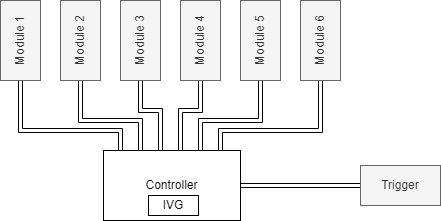
\includegraphics[width=10cm]{./Figures/concept_all.png}
    \caption{Basic layout of the three components controller, trigger and modules.}
    \label{fig:concept}     
\end{figure}

\noindent The system operates by the fire-and-forget principle, by which the user arms both the controller and the trigger and after pressing the trigger button the controller will automatically ignite the firework in the programmed sequence. No user input is needed after setting off. When the trigger is pressed the system goes into a $10s$ delay phase in order for the user to get to safety. After the delay phase is finished, the ignition phase is entered, where the programmed sequence will play through until the predetermined endpoint is reached. The trigger can be replaced with a RF-trigger although this is not recommend due safety and legal concerns in some countries. The delay period also serves as a fail safe, because if the system is triggered by accident, the user is able to abort the start by disarming the system. During the ignition phase it is also possible to halt the program by disarming the system, although re-triggering will go through the delay phase again.\\

\noindent The ignition sequence is programmed by USB via serial communication(See \cref{USB Connection}). Programming the sequence can be accomplished by directly connecting to the serial port and typing the commands by hand or by using the Software provided(See \cref{Software}).\\

\noindent As the device is most likely placed in open-air field there is no way for it to be power by mains power, therefore it has to be powered by batteries. However, the usage of rechargeable batteries or LiPo-batteries was not desirable for this project, due cost issues and the additional requirement of protection circuits. A better alternative was found by using common $5V$ powerbanks for smart phones. Those already provide steady $5V$ with build-in protective mechanisms. Furthermore, nowadays many people use powerbanks and if the user forgets to charge or forgets the powerbank altogether, there is a high chance some will be able to provide one as replacement. A powerbank can be charged by a simple micro USB cable which is also very common and removes the need for a specialized charger.





\pagebreak

\section{Hardware}
\label{Hardware}

As already explained in \cref{Concept}, the device is split into three parts. This section will explore each part separately by looking into the design choices that were made. Although the controller is described as one unit, in reality consist  of to distinct circuits. One is the ignition voltage generator (See \cref{Ignition Voltage Generator}) which is responsible for generating the voltage/charge that is necessary for setting off the bridge wire detonators. The other circuit is the control logic that does the controlling (See \cref{Controller}).


\subsection{The Ignition Voltage Generator}
\label{Ignition Voltage Generator}

\begin{figure}[!ht]
    \centering
    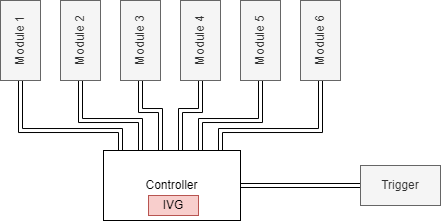
\includegraphics[width=5cm]{./Figures/concept_ivg.png} 
\end{figure}

\noindent The step-up convert shown in \Cref{fig:ivg_circuit} works by the basic principle of a step-up/boost converter by storing energy in form of a magnetic field inside a inductor and releasing the energy as a current into a capacitor. Repeat this process at high frequency and a higher voltage is created at the output compared to the input voltage. For a better explanation see the document about this topic by \textit{Texas-Instruments}\footnote{\url{https://www.ti.com/lit/an/snva731/snva731.pdf}}.


\subsubsection{Circuit}

\begin{figure}[!ht]
    \centering
    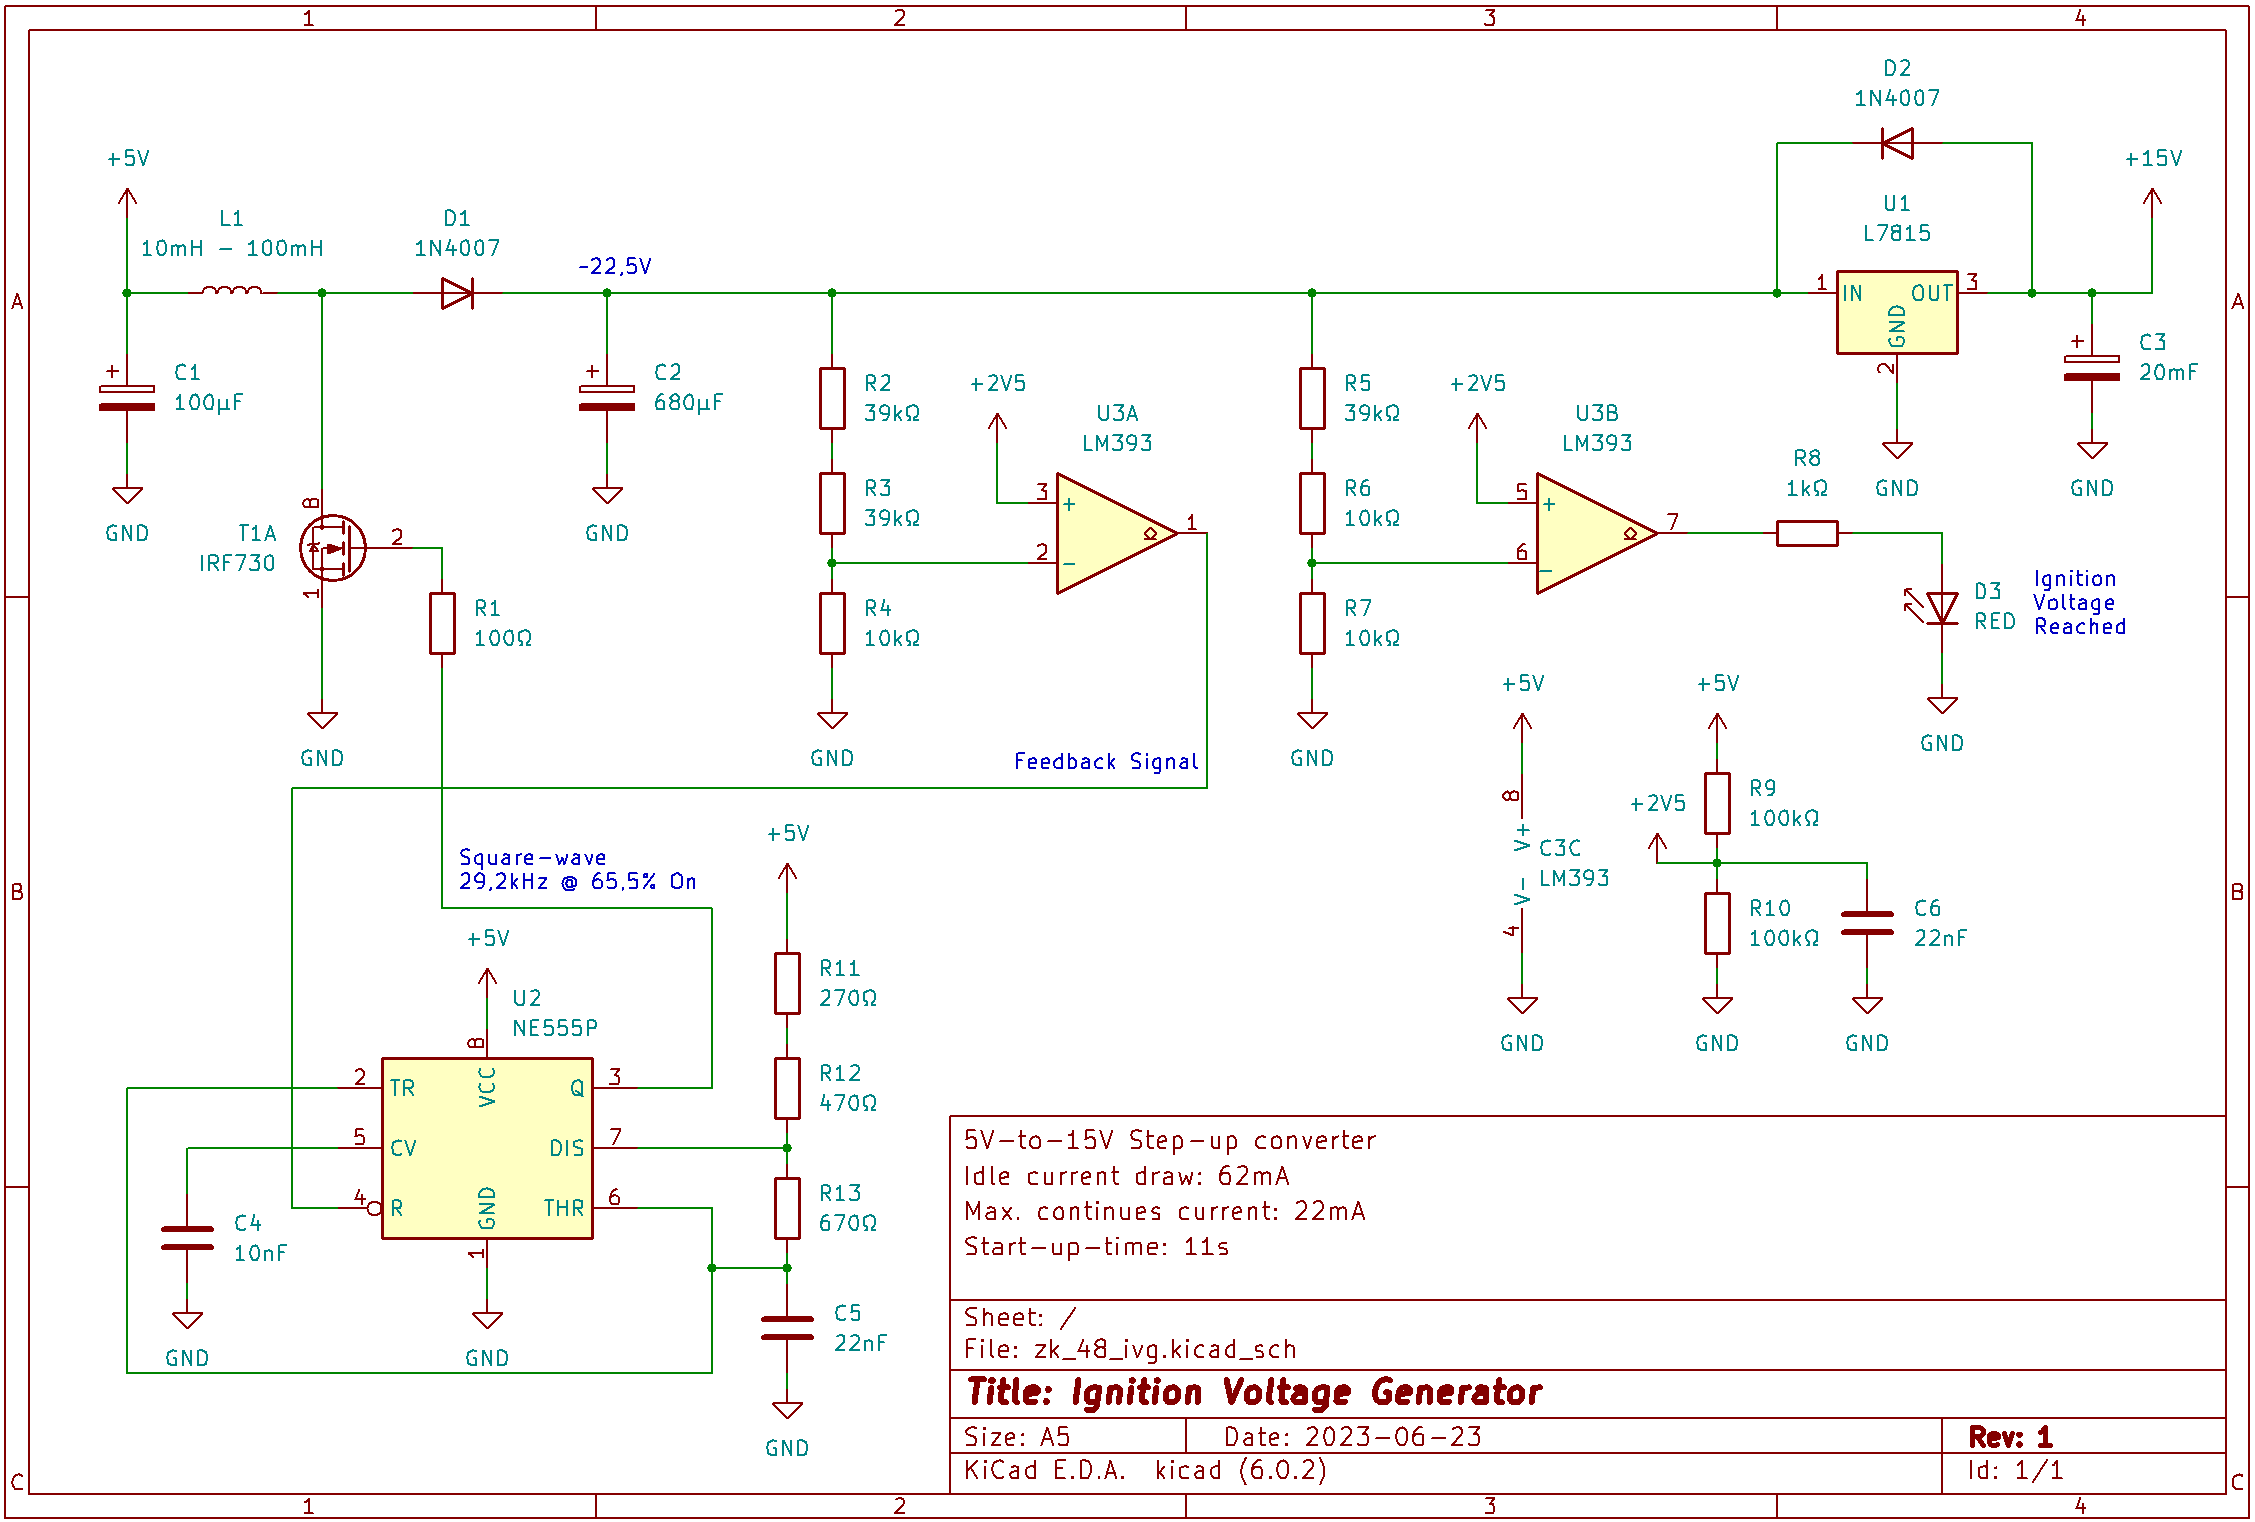
\includegraphics[width=15cm]{./Figures/ivg_circuit.png}
    \caption{Circuit of the step-up converter that generates 15V DC for the ignition voltage}
    \label{fig:ivg_circuit}     
\end{figure}

\pagebreak

\subsubsection{How does the circuit work?}

\noindent The circuit shown in \Cref{fig:ivg_circuit} contains the popular NE555\footnote{\url{ https://www.ti.com/lit/ds/symlink/ne555.pdf}}, the dual comparator LM393\footnote{\url{https://www.ti.com/lit/ds/symlink/lm393.pdf}} and a fixed $15V$ linear voltage regulator L7815\footnote{\url{https://www.st.com/resource/en/datasheet/l78.pdf}}. The NE555 is used as a square wave oscillator to generate a $29,2kHz$ $5V_{pp}$ signal with a $65,5\%$ on-time. This signal drives the IRF730\footnote{\url{https://www.vishay.com/docs/91047/91047.pdf}} N-channel MOSFET, which switches current through the inductor $L1$ and therefore charging the capacitor $C2$ an creating a voltage. We shall name this voltage the intermediate voltage.\\

\noindent Through a voltage divider the voltage at $C2$ is stepped down by a factor of $\frac{1}{9}$ and compared to a $2,5V$ reference voltage by $U3A$. This results in a $5V$ output signal at the output of $U3A$, if the capacitors $C2$ voltage is lower than $22,5V$. This signal is called the feedback signal with turns off the NE555 if the intermediate voltage has reached $22,5V$. Using schmitt-trigger would result in a oscillating turning off and on of the feedback signal which is undesirable in this configuration. If the intermediate voltage reaches $22,5V$, the feedback signal will no longer be $5V$ or $0V$, rather it will drop to a constant $2,5V$. This is expected, but will result in a unpredictable behaviour at the NE555, which expects a binary reset signal. This seems like a problem, but in reality will result in the NE555 output voltage to drop below the on-voltage of the IRF730, thus turning it off. It is also observable that the frequency and on-time of the NE555 output is rising, but this does not matter, because the voltage already dropped significantly. \\

\noindent The intermediate voltage is then converted by the L7815 to stable $15V$ which charges the large $20mF$ ignition capacitor $C3$. This voltage is called the ignition voltage.\Cref{eq:power_in_system} calculates the energy stored in the complete system with all six modules connected (Thus the total capacitance being $26mF$, but read more in \Cref{Module}) which equates to around $3J$ and therefore not presenting any harm or danger to life\footnote{\url{https://www.ehss.vt.edu/programs/ELR_capacitors.php}}. Touching fully charged capacitors with wet hands did not result in any shock or pain.\\

\begin{equation}
W_{el}=\frac{U^2 \cdot C_{tot}}{2}=\frac{(15V)^2 \cdot 26mF}{2}=2,925J
\label{eq:power_in_system}
\end{equation}\\

\noindent The second comparator $U3B$ in the LM393 package was used to turn on a red LED $D3$ whose purpose is to indicate whether the intermediate voltage is bigger than $14,75V$. This shows the user if the system is ready for operation and if a ignition voltage is present.\\


\noindent \small{\textit{Note: Please note that the ignition voltage generator was designed by the author and is by no means ideal nor optimized. This was the first attempt at creating a step-up convert from scratch with components that were on hand. It does the job well (See \cref{Testing}), but any bought step-up convert will do just fine and most likely better.}}\\

\pagebreak

\subsubsection{Testing}
\label{Testing}
For testing the ignition voltage generator displayed in \Cref{fig:ivg_circuit}, a resistor with $4,7\Omega$ was placed into port 1 on module 1. This resistance is equal to two bridge wire detonators in series. This makes sure the system is tested in an less than ideal situation, because typically only one would be used. \Cref{fig:testrig_pulse} shows the complete test setup, with the pulse generator symbolically representing the controller. The system was programmed to fire port 1 on module 1 eight times with a $10ms$ delay between each pulse.

\begin{figure}[!ht]
    \centering
    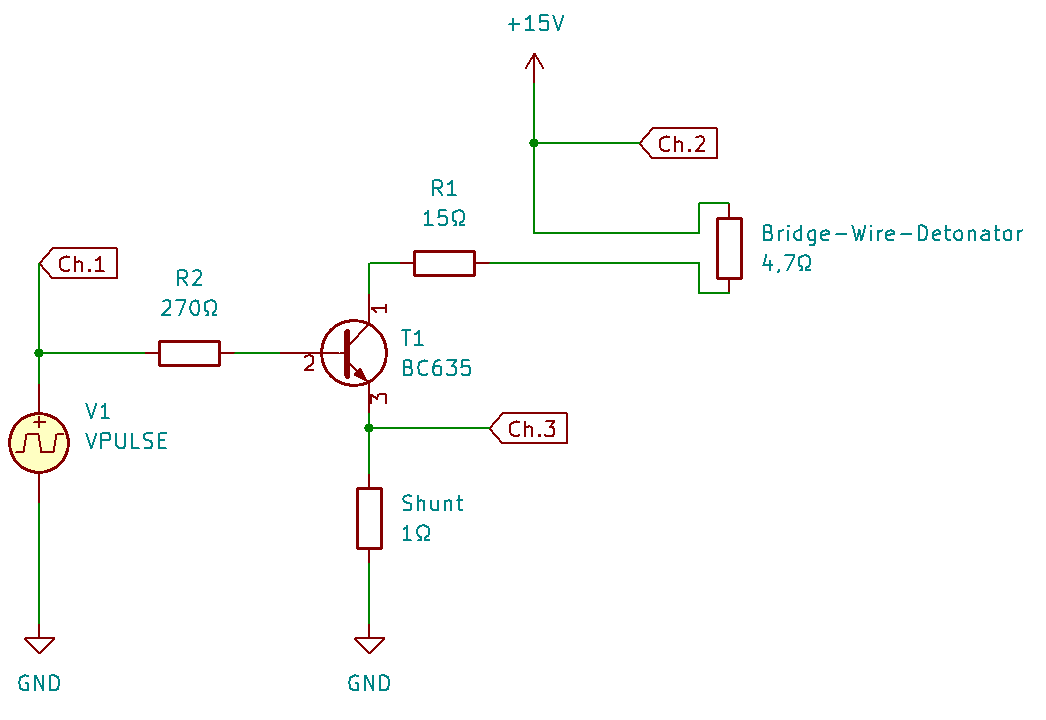
\includegraphics[width=7cm]{./Figures/testrig_pulse.png}
    \caption{Circuit for testing stability of ignition voltage and current though a simulated bridge wire detonator.}
    \label{fig:testrig_pulse}     
\end{figure}

\paragraph{Results}
\label{Results}

\noindent The first test consisted of 8 pulses to simulate fast consecutive firing of pyrotechnic single-shots\footnote{\url{https://www.youtube.com/watch?v=UgVG9NcA5CM}} or other pyrotechnic effects. Normally firing the same port multiple times does not make sense, but for testing purposes this is equivalent to firing eight separate ports. The resulting waveform was captured with the Quad DSO (digital storage oscilloscope) \textit{Rigol DS1054z}\footnote{\url{https://www.batronix.com/pdf/Rigol/UserGuide/DS1000Z_UserGuide_EN.pdf}}.\\

\begin{figure}[!ht]
    \centering
    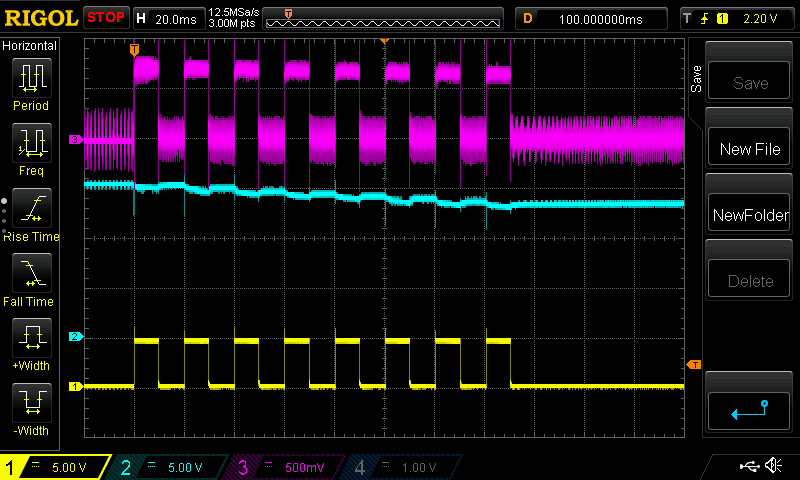
\includegraphics[width=10cm]{./Figures/eight_pulses_close.png}
    \caption{Oscilloscope recorded waveforms of eight pulses in close up.}
    \label{fig:eight_pulses_close}     
\end{figure}
 
\noindent The main objective of this test is to confirm that rapid firing does not affect the system ability to ignite further detonators. This can evidently be confirmed by looking at the curve of Ch.3 and Ch.2 in \Cref{fig:eight_pulses_close}. The ignition voltage is represented by Ch.2 which drops by only $2V$, thus being neglect able. By looking at Ch.3, which shows the current through the bridge wire detonator, its clearly recognizable that current is above $700mA$, even at the last pulse. Past testing showed, bridge wire detonators already ignite at around $300mA-400mA$. This confirms the efficacy and the systems ability to continuously ignite pyrotechnic effects at a high rate.

\pagebreak


\begin{figure}[!ht]
    \centering
    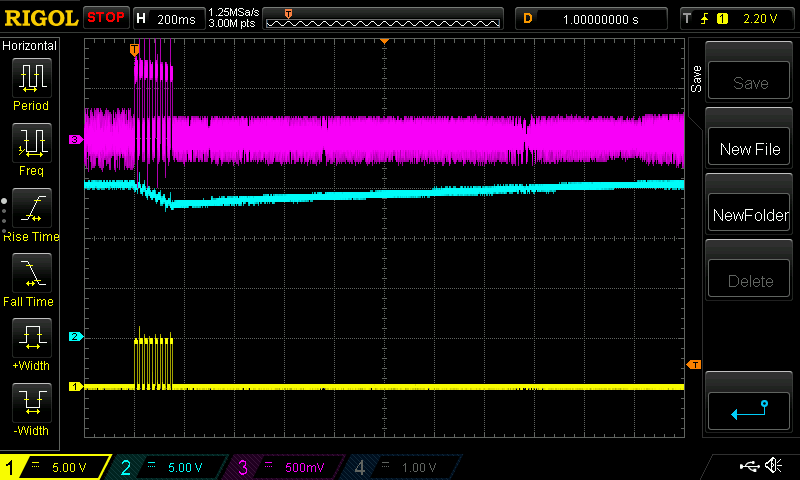
\includegraphics[width=10cm]{./Figures/eight_pulses_wide.png}
    \caption{Oscilloscope recorded waveforms of eight pulses until returning to $15V$.}
    \label{fig:eight_pulses_wide}     
\end{figure}

\noindent In \Cref{fig:eight_pulses_wide} the time was measured for the ignition voltage to return back to $15V$ after firing eight times. This time amounts to about $2s$ which is acceptable but could be better.\\ 

\noindent The third test focused in finding the absolute limit of the system. To achieve this objective the ZK-48 was programmed to use all its 48 sequence slots and fire port 1 on module 1 48 times. 

\begin{figure}[!ht]
    \centering
    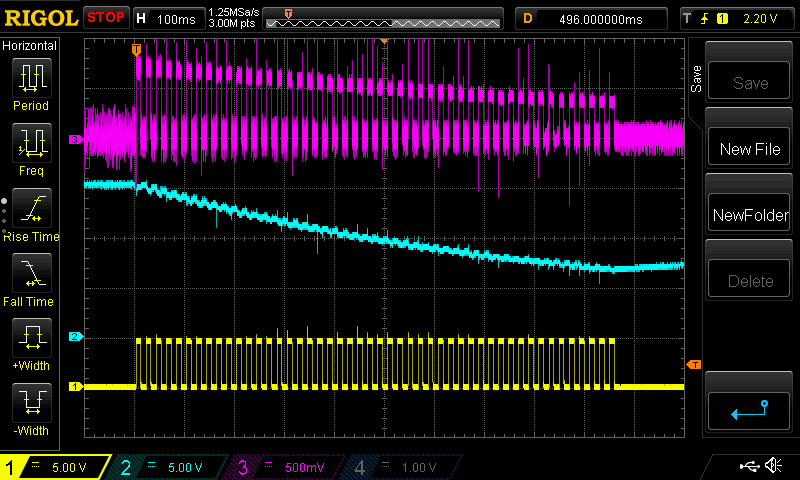
\includegraphics[width=10cm]{./Figures/max_pulses.png}
    \caption{Oscilloscope recorded waveforms of 48 fire pulses.}
    \label{fig:max_pulses}     
\end{figure}

\noindent The number of maximal fire pules was determined by counting the number of pulses until the current through the detonator fell below $500mA$. This current value was chosen arbitrary, as it is the average between the lowest recorded current at which a detonator ignites($300mA$) and the current at the first ignition pulse($700mA$). By this definition the maximal number of consecutive fire pulses is about 24.

\paragraph{Conclusion}
The ignition voltage generator is able to provide a steady voltage even under load(See \Cref{fig:testrig_pulse}) and is able to ignite 24 bridge wire detonators with $10ms$ delay. This is just theoretical and needs to be confirmed with real detonators, however this is already promising to conclude proper operation. Although the generator performs well it has many flaws and should be subject of rigorous optimization. For example the ignition voltage should ideally not drop at all and remain steady even if continues $700mA$ are drawn. By using a bought step-up converter with proper control logic, such as current regulation, instead of a simple feedback loop, most problems would be rectified. The projects goal is not to buying electronic modules and soldering them together, instead this is an exploration of circuit design and should be viewed as a learning experience.


\pagebreak


\subsection{Controller}
\label{Controller}

\begin{figure}[!ht]
    \centering
    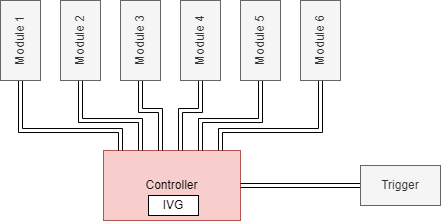
\includegraphics[width=5cm]{./Figures/concept_controller.png} 
\end{figure}

\noindent The controller is responsible for interpreting all user inputs such as the arm switch and the trigger signal which are processed by the µC to correctly control all modules and controlling the status LED.  The ignition voltage generator is also soldered on the physical circuit board together with the controller, but more about that in \Cref{Circuitboard}.

\subsubsection{Circuit}

\begin{figure}[!ht]
    \centering
    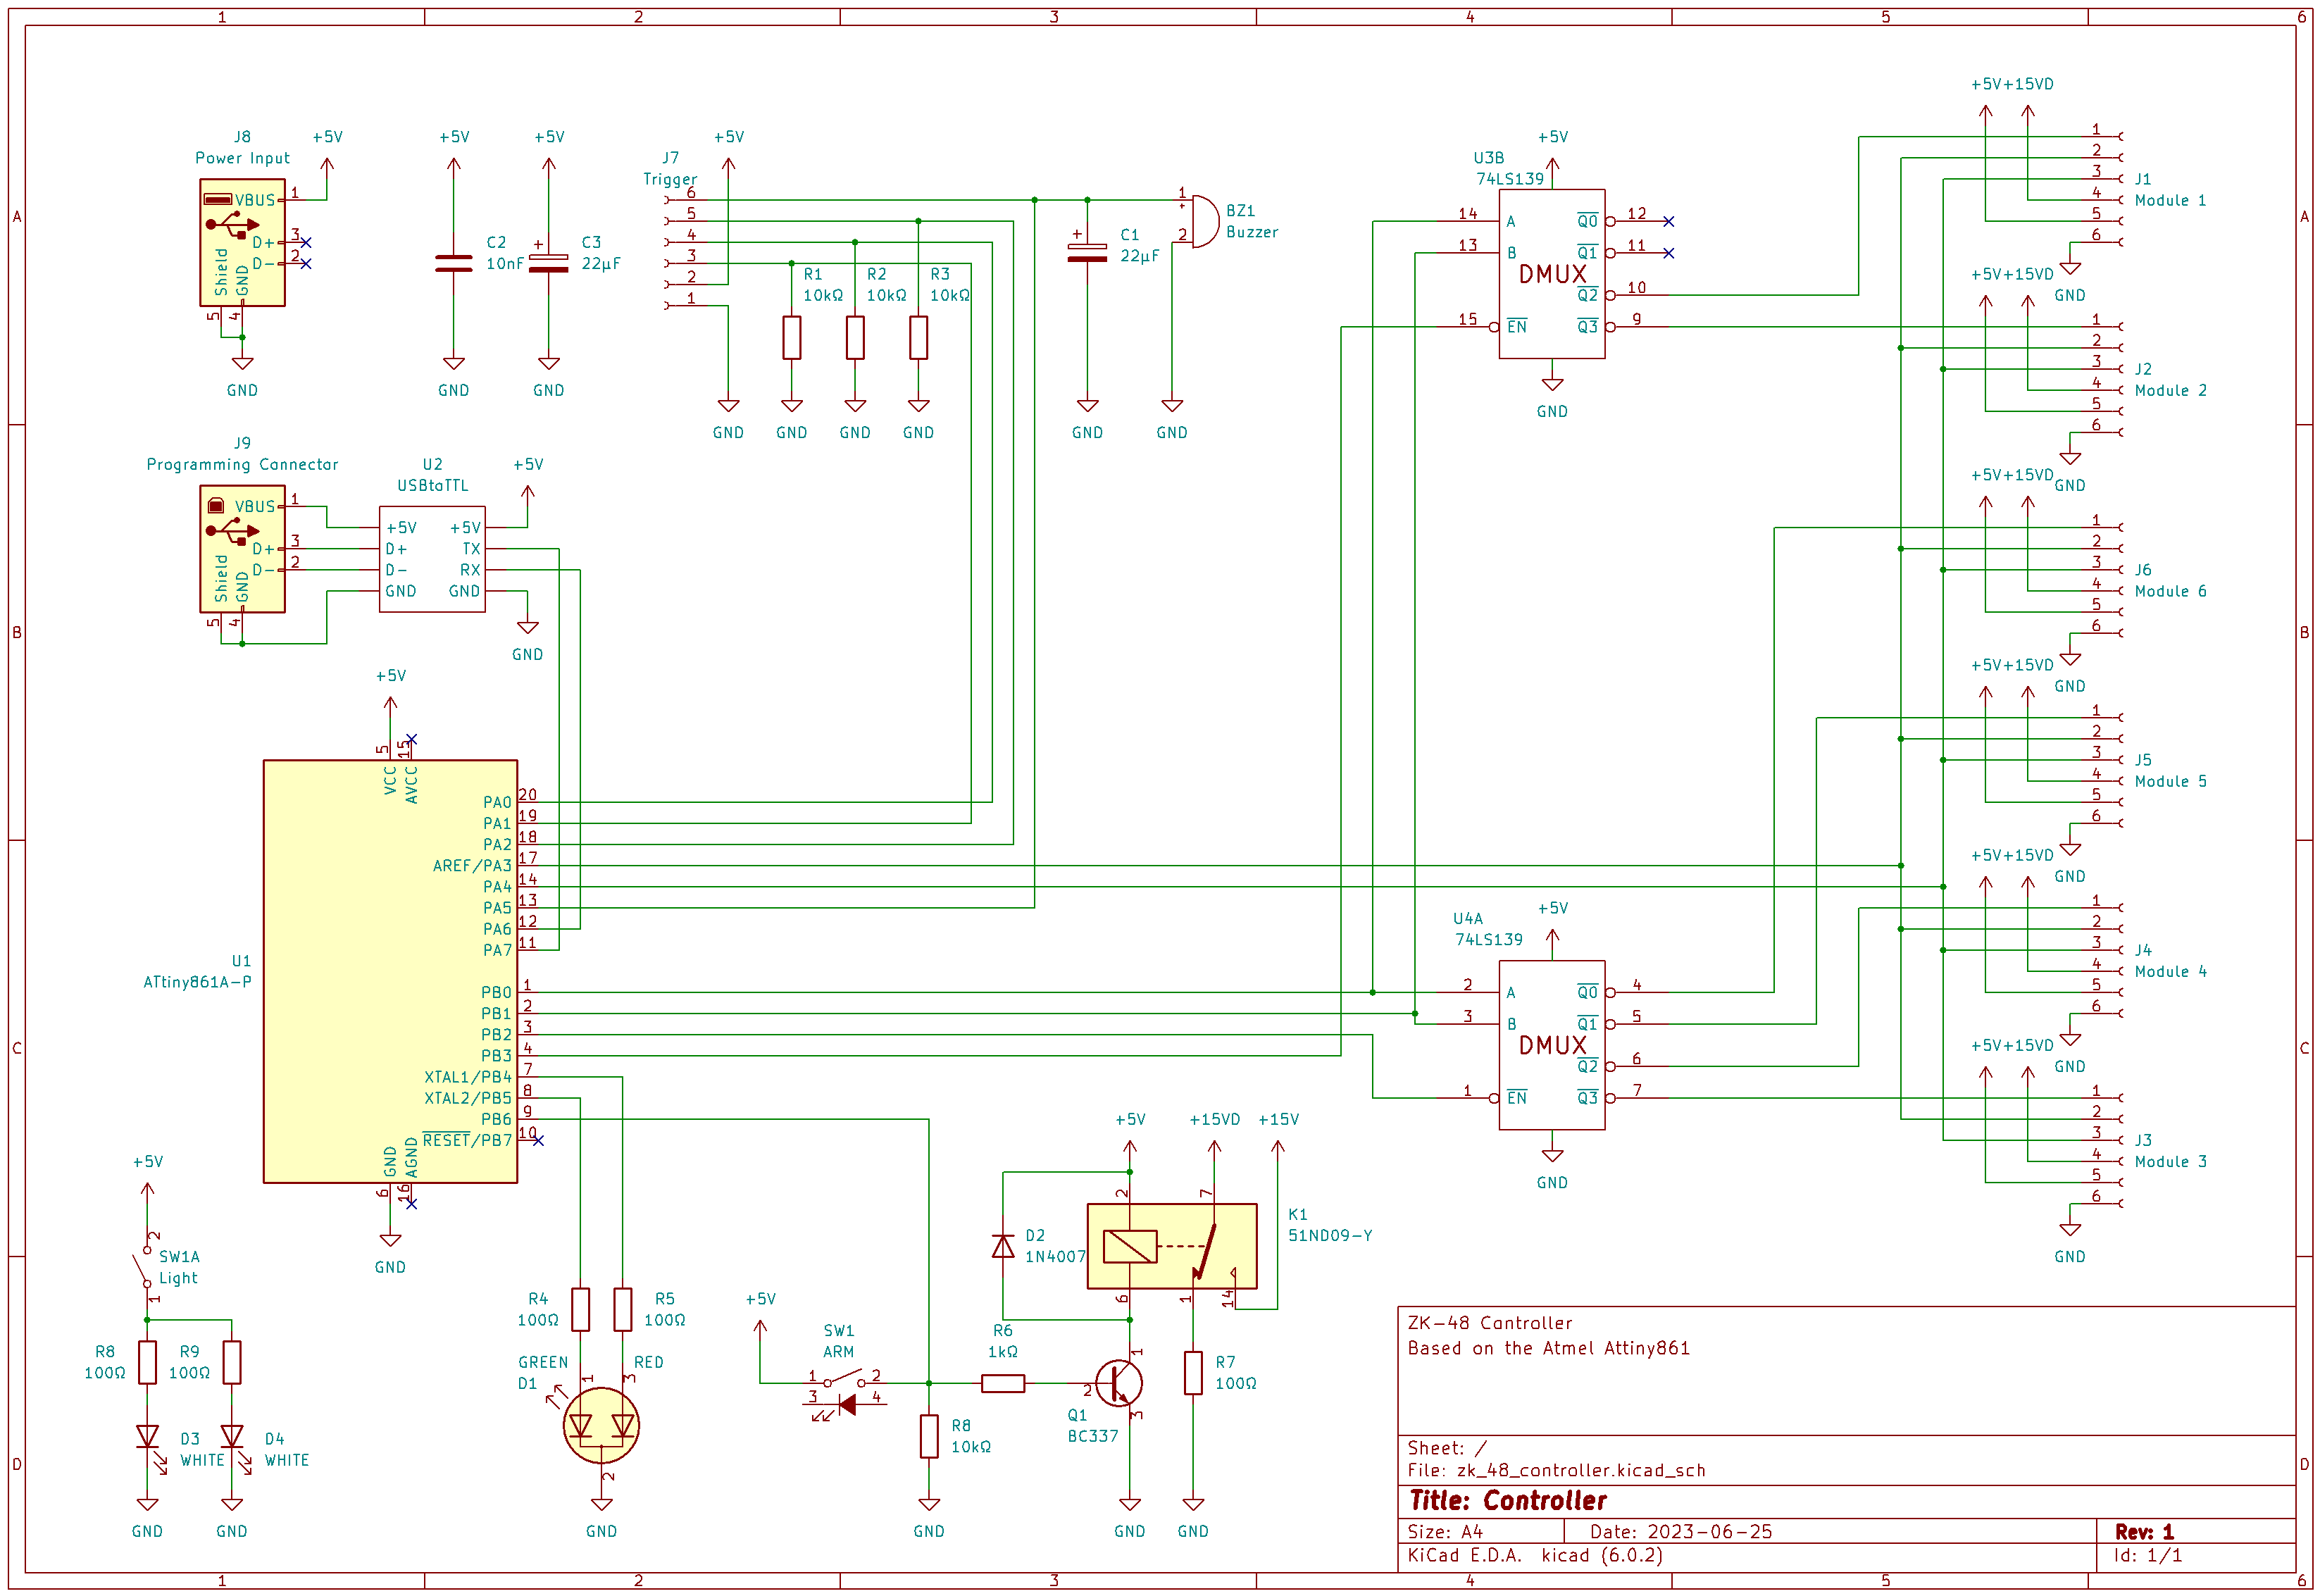
\includegraphics[width=15cm]{./Figures/controller_circuit.png}
    \caption{Circuit of the controller without ignition voltage generator.}
    \label{fig:controller_circuit}     
\end{figure}

\pagebreak

\subsubsection{Components of the Controller}
\label{Components of the Controller}
The controller consist of the peripheral managing and controlling logic, the USB serial communication and the arm safety circuit. 

\paragraph{Peripheral Managing and Controlling Logic}
This part of the circuit is located on the right side of the circuit depicted in \Cref{fig:controller_circuit}. Its purpose is the selection of the correct module to fire. To understand how this works its important to first explain how the µC fires a port on a module.\\

\noindent In \Cref{fig:controller_circuit} notice that all module sockets DATA and CLK lines are connected together(For the pin-out see \Cref{Socket and Plugs}). The µC first serially transmits to all modules shift registers(See \Cref{none}) what port is about to be fired. In the second step the µC will select one out of the six modules which then fires the port that was set in the first step.\\


\noindent The selection process is accomplished by two demultiplexer $U4A$ and $U3B$ which are both contained in the dual DMUX 74LS139\footnote{\url{https://www.ti.com/lit/ds/symlink/sn54ls139a-sp.pdf}}. Instructions are given to the DMUX by the µC. Circuit design only allows to select one module at a time. Thus the system being unable to fire to ports on different modules at the same time. Currently firmware does not support simultaneous firing of to ports anyway. This is a disadvantage, but is manageable by programming the system to fire two ports with no delay, which results in a $10ms$ between each firing. Our human eyes cannot pick up on such short delays and pyrotechnic is also not timed perfectly, therefore this does not impose a big problem.\\

\noindent The socket of the external trigger also falls into peripheral circuitry, but  it does not contain any real logic. Resistors $R1-R3$ pull down the sockets FIRE, ARMED and CONCD lines(For the pin-out see \Cref{Socket and Plugs}). Those are inputs of the µC and are able to not have a defined potential if the user unplugs the trigger when the system is powered, therefore needing to be pulled down. The local signal buzzer $BZ1$ is wired to the sockets BUZZER signal and its voltage is stabilized with the capacitor $C1$.\\


\paragraph{USB serial communication}
For programming the µC has to communicate with a computer. This is the only bought circuit of this project because the Attiny861 does not have a build-in UART communication and no FTDI or other UART-to-TTL chip was easily and cheaply obtainable. Therefore the decision was made to save time and money by buying a UART-to-TTL module of \textit{Amazon}. \\

\begin{figure}[!ht]
    \centering
    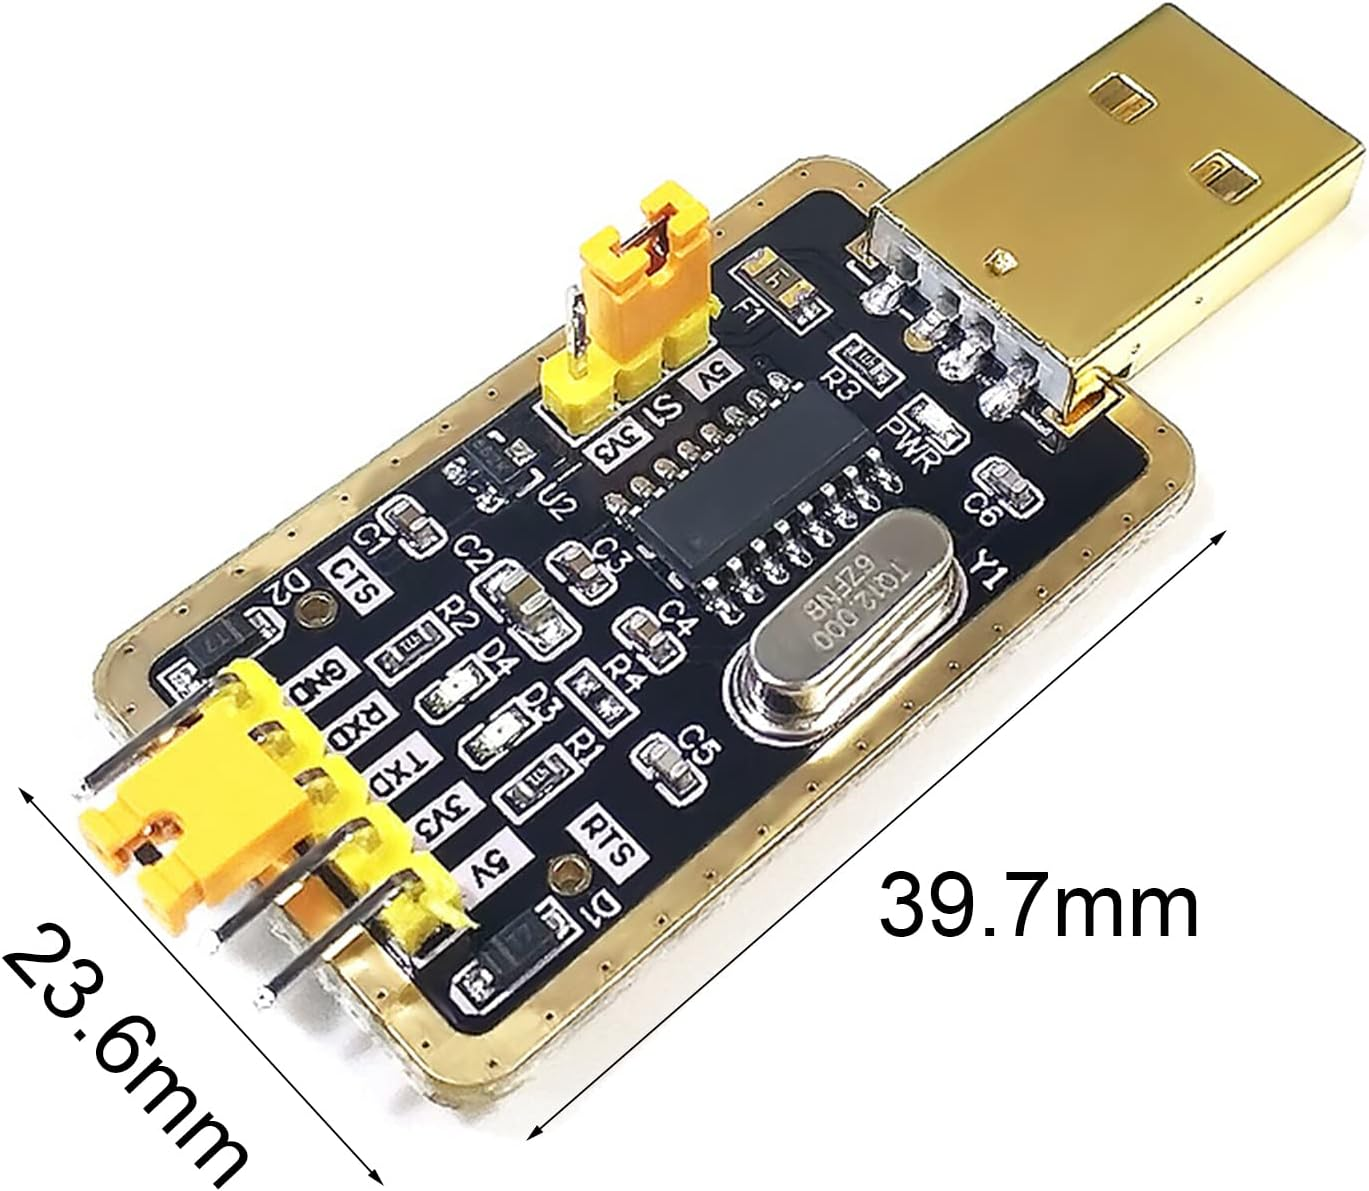
\includegraphics[width=4cm]{./Figures/uart_ttl.jpg}
    \caption{The bought UART-to-TTL converter from \textit{Amazon}}
    \label{fig:uart_ttl}     
\end{figure}

\noindent The module depicted in \Cref{fig:uart_ttl} and the image rights belongs to \textit{Amazon}\footnote{\url{https://amzn.eu/d/3QKPgB9}}.\\


\pagebreak

\paragraph{Arm safety circuit}
This part of the controller circuit is shown in \Cref{fig:controller_circuit} on the bottom. For safety reasons, the ignition voltage is galvanically disconnected from the ignition voltage line of the modules, if the system is unarmed. Without this circuit, it is possible for a bridge wire detonator to ignite prematurely during power up or if a module is disconnected and reconnected. \\
\noindent The cause of this dangerous behaviour is explained by the shift registers inside of the modules. Most if not all shift registers when connected to power will take on random values inside their registers. If the output is disabled through the \textit{Output Enable} pin on the 74HC595, this could not happen. However those enable pins are driven by the DMUX on the controller (See \Cref{fig:controller_circuit}) and those DMUX are controlled by the µC which takes more time to boot than the shift registers. Thus for a very short period ($<20µs$) turning on the some of the shift registers outputs and making it possible for a false ignition. Although this cannot be prevented, it is possible to take away the ignition voltage and pulling down the modules ignition voltage line with a $100\Omega$ resistor (See resistor $R7$ in \Cref{fig:controller_circuit}). Relay $K1$ is only connecting the ignition voltage to the modules power lines if the system is armed and therefore making it impossible to accidentally set of pyrotechnics prematurely.

\paragraph{Additional circuits}
As the system will most likely be operated in the dark, the decision was made to add a small LED light inside the casing of the complete controller to illuminate the interface. The circuit can be found in the bottom left corner in \Cref{fig:controller_circuit}, although the LEDs are not soldered onto the circuit-board. They are place inside of the lid, thus shining downwards onto the interface if the case is opened.

\subsubsection{Socket and Plugs}
\label{Socket and Plugs}

\begin{figure}[!ht]
    \centering
    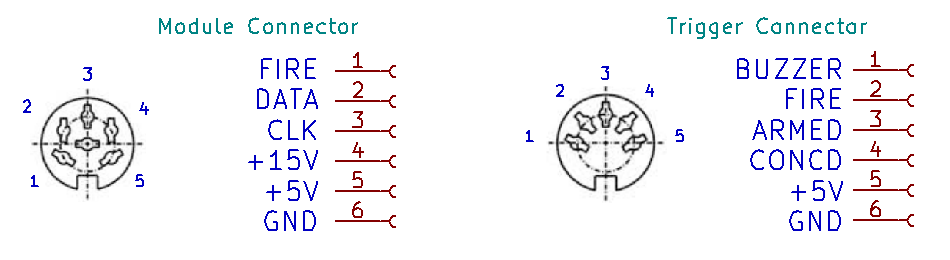
\includegraphics[width=10cm]{./Figures/mod_trig_connector.png}
    \caption{The pin-out of the trigger and modules socket/plug.   }
    \label{fig:mod_trig_connector}     
\end{figure}

\noindent The symbols in black visible in \Cref{fig:mod_trig_connector} of the socket belong to \textit{reichelt.de}\footnote{\url{https://cdn-reichelt.de/documents/datenblatt/C160/MAB\%205S-ROHS_XX.pdf}}\\

\noindent To connect the peripheral devices to the controller DIN\footnote{\url{https://en.wikipedia.org/wiki/DIN_connector}} plugs and sockets were used. The modules socket and plug where chosen differently than the triggers, because plugging in the trigger into a module socket would damage the triggers electronics. For the pin-out of each socket see \Cref{fig:mod_trig_connector} and below in \Cref{fig:din_plug_socket} the modules socket and plug is visible.

\begin{figure}[!ht]
    \centering
    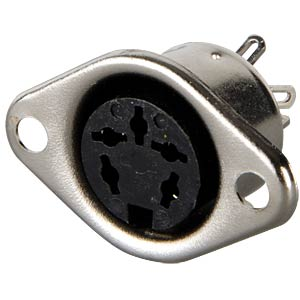
\includegraphics[width=3cm]{./Figures/MAB_5.jpg}
    \hspace{2cm}
    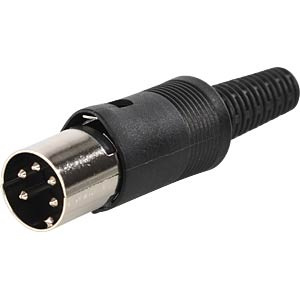
\includegraphics[width=3cm]{./Figures/MAS_50.jpg}
    \caption{DIN socket and plug of the modules.}
    \label{fig:din_plug_socket}     
\end{figure}

\noindent The images visible in \Cref{fig:din_plug_socket} of the socket and plug belong to \textit{reichelt.de}\footnote{\url{https://cdn-reichelt.de/bilder/web/xxl_ws/C160/MAS_50.png}} \footnote{\url{https://cdn-reichelt.de/bilder/web/xxl_ws/C160/MAB_5.png}}\\

\pagebreak

\subsubsection{Circuit board}
\label{Circuitboard}

\begin{figure}[!ht]
    \centering
    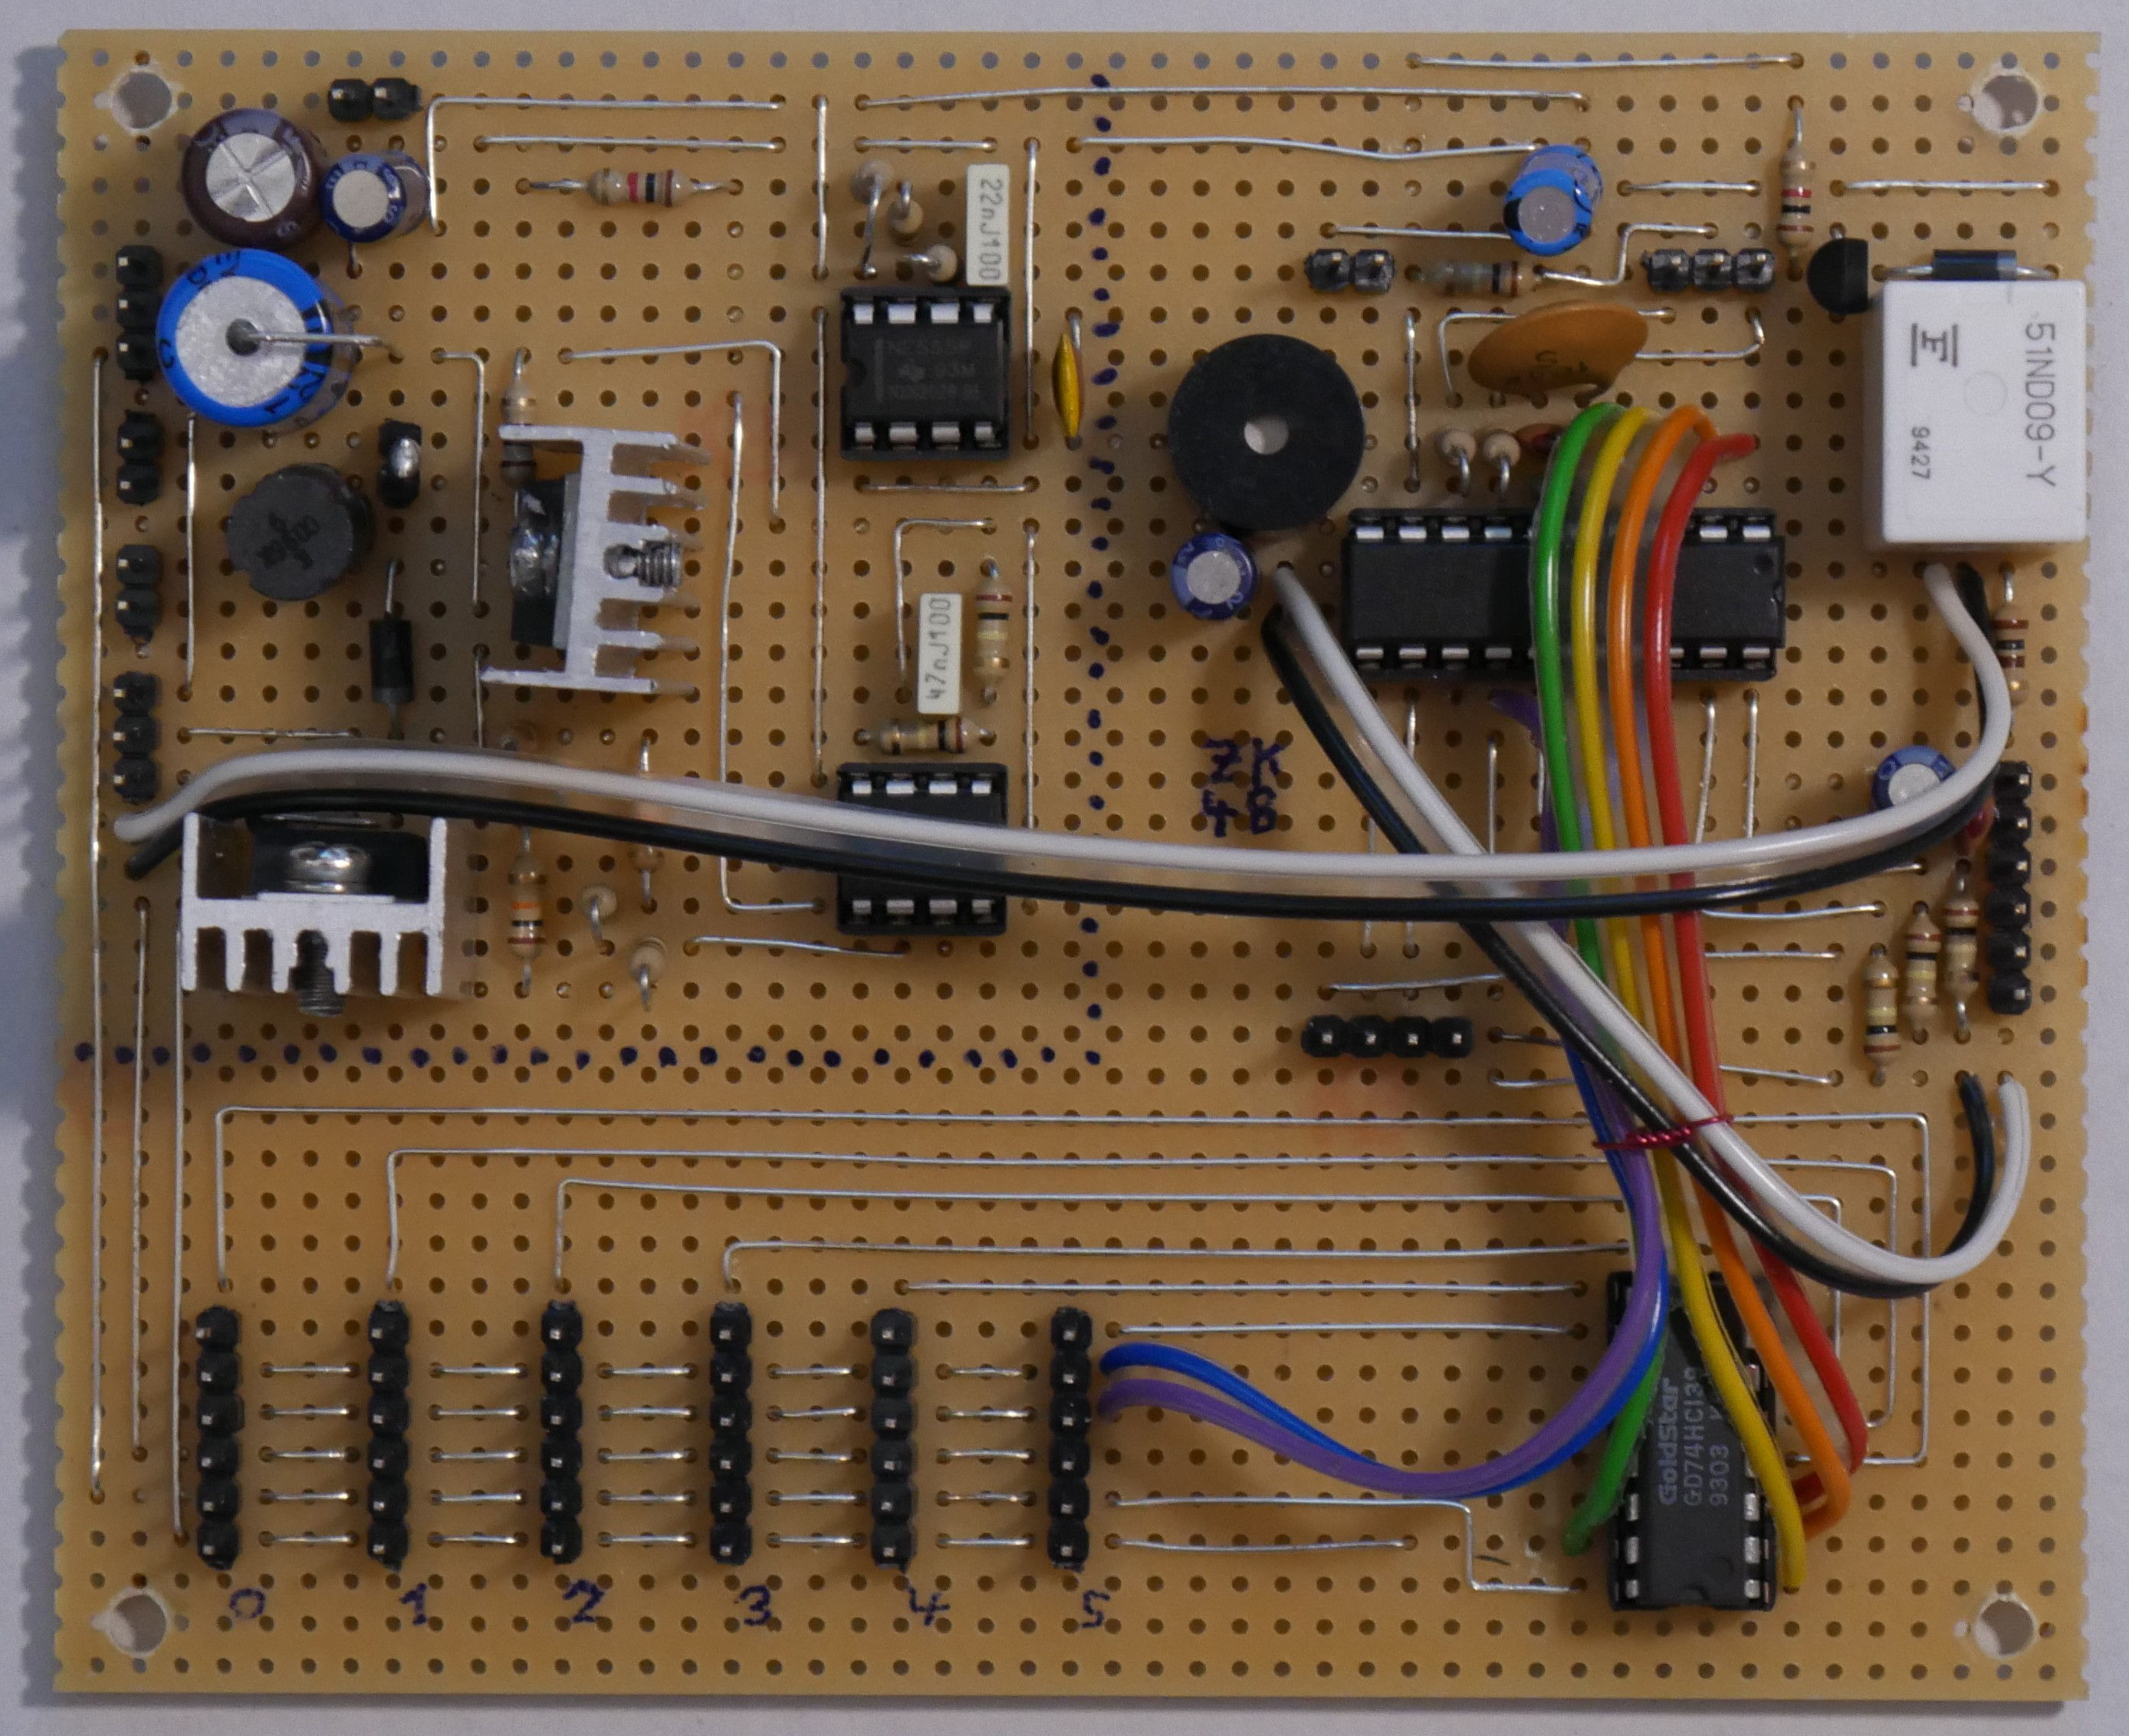
\includegraphics[width=10cm]{./Figures/controller_circuit_soldered.JPG}
    \caption{The controller circuit (See \Cref{fig:controller_circuit}) and the ignition voltage generator (See \Cref{fig:ivg_circuit}) soldered onto a perfboard.   }
    \label{fig:controller_circuit_soldered}     
\end{figure}

\noindent A perfboard with one sided copper solder pads and the dimensions 100x115mm was used as the base for the controller circuit. Both the controller circuit (See \Cref{fig:controller_circuit}) and the ignition voltage generator (See \Cref{fig:ivg_circuit}) was soldered onto this board. Ideally this should be a PCB, but this would make it hard to change things in the future. \\

\noindent In the left top corner the ignition voltage generator is visible with heat sinks on the linear voltage regulator and MOSFET. The right top corner contains the µC, all the pin-headers for connecting the switches and LEDs as well es the arm safety circuit. On the bottom the peripheral managing logic is visible together with the six pin-headers for the modules.

\pagebreak

\subsubsection{Housing of the Controller}
\label{Housing of the Controller}

\begin{figure}[!ht]
    \centering
    \includegraphics[width=10cm]{./Figures/controller_plate_top.JPG}
    \caption{ The circuit board depicted in \Cref{fig:controller_circuit_soldered} mounted and wired onto the backside of the devices interface. }
    \label{fig:controller_plate_top}     
\end{figure}

\noindent The image in \Cref{fig:controller_plate_top} shows the controller with all peripheral devices connected. On the top are the two big capacitors that store the ignition and intermediate voltage, secured to the board by a metal band.\\

\begin{figure}[!ht]
    \centering
    \includegraphics[width=10cm]{./Figures/controller_plate_side.JPG}
    \caption{ The circuit board depicted in \Cref{fig:controller_circuit_soldered} mounted and wired onto the backside of the devices interface viewed from the side. }
    \label{fig:controller_plate_side}     
\end{figure}

\noindent As the baseplate for the interface, a $2cm$ thick wooden plate was used. Holes were drilled to allow switches, status LED and the sockets to be mounted. Then the plate was painted black and everything was screwed on. In \Cref{fig:controller_plate_side} the controller circuit board is shown mounted by $1,5cm$ four standoffs. For wiring ribbon cables  were used to connect the switches and other input or output items. The sockets of the trigger and modules were wired to the controller circuit by a 5-line telephone cable\footnote{\url{https://amzn.eu/d/65ZALnq}} with shielding. This cable was also the choice for externally connecting the trigger and modules to the interface.   

\pagebreak

\begin{figure}[!ht]
    \centering
    
\includegraphics[width=4cm]{./Figures/gn_case.jpg}
    \caption{ The gun case used for housing the controller. }
    \label{fig:gn_case}     
\end{figure}

\noindent The image of the gun case visible in \Cref{fig:gn_case} belongs to \textit{Amazon}\footnote{\url{https://amzn.eu/d/eWSlyFs}}\\

\noindent A gun case was bought of \textit{Amazon} (See \Cref{fig:gn_case}), and the cushioning in the lower part of the case was removed to make room for the controller. The complete contorller interface was put into a case and screwed from the sides. \Cref{fig:controller_open} depicts the finished controller turned on. The earlier mentioned lighting(See \Cref{Components of the Controller} "Additional circuits") was installed in to top part of the case and the wires were hiden behind the cushioning. In \Cref{fig:controller_open} the wires can be seed coming from the top part of the case going to the lower part(See \Cref{fig:controller_open} right top corner).


\begin{figure}[!ht]
    \centering
    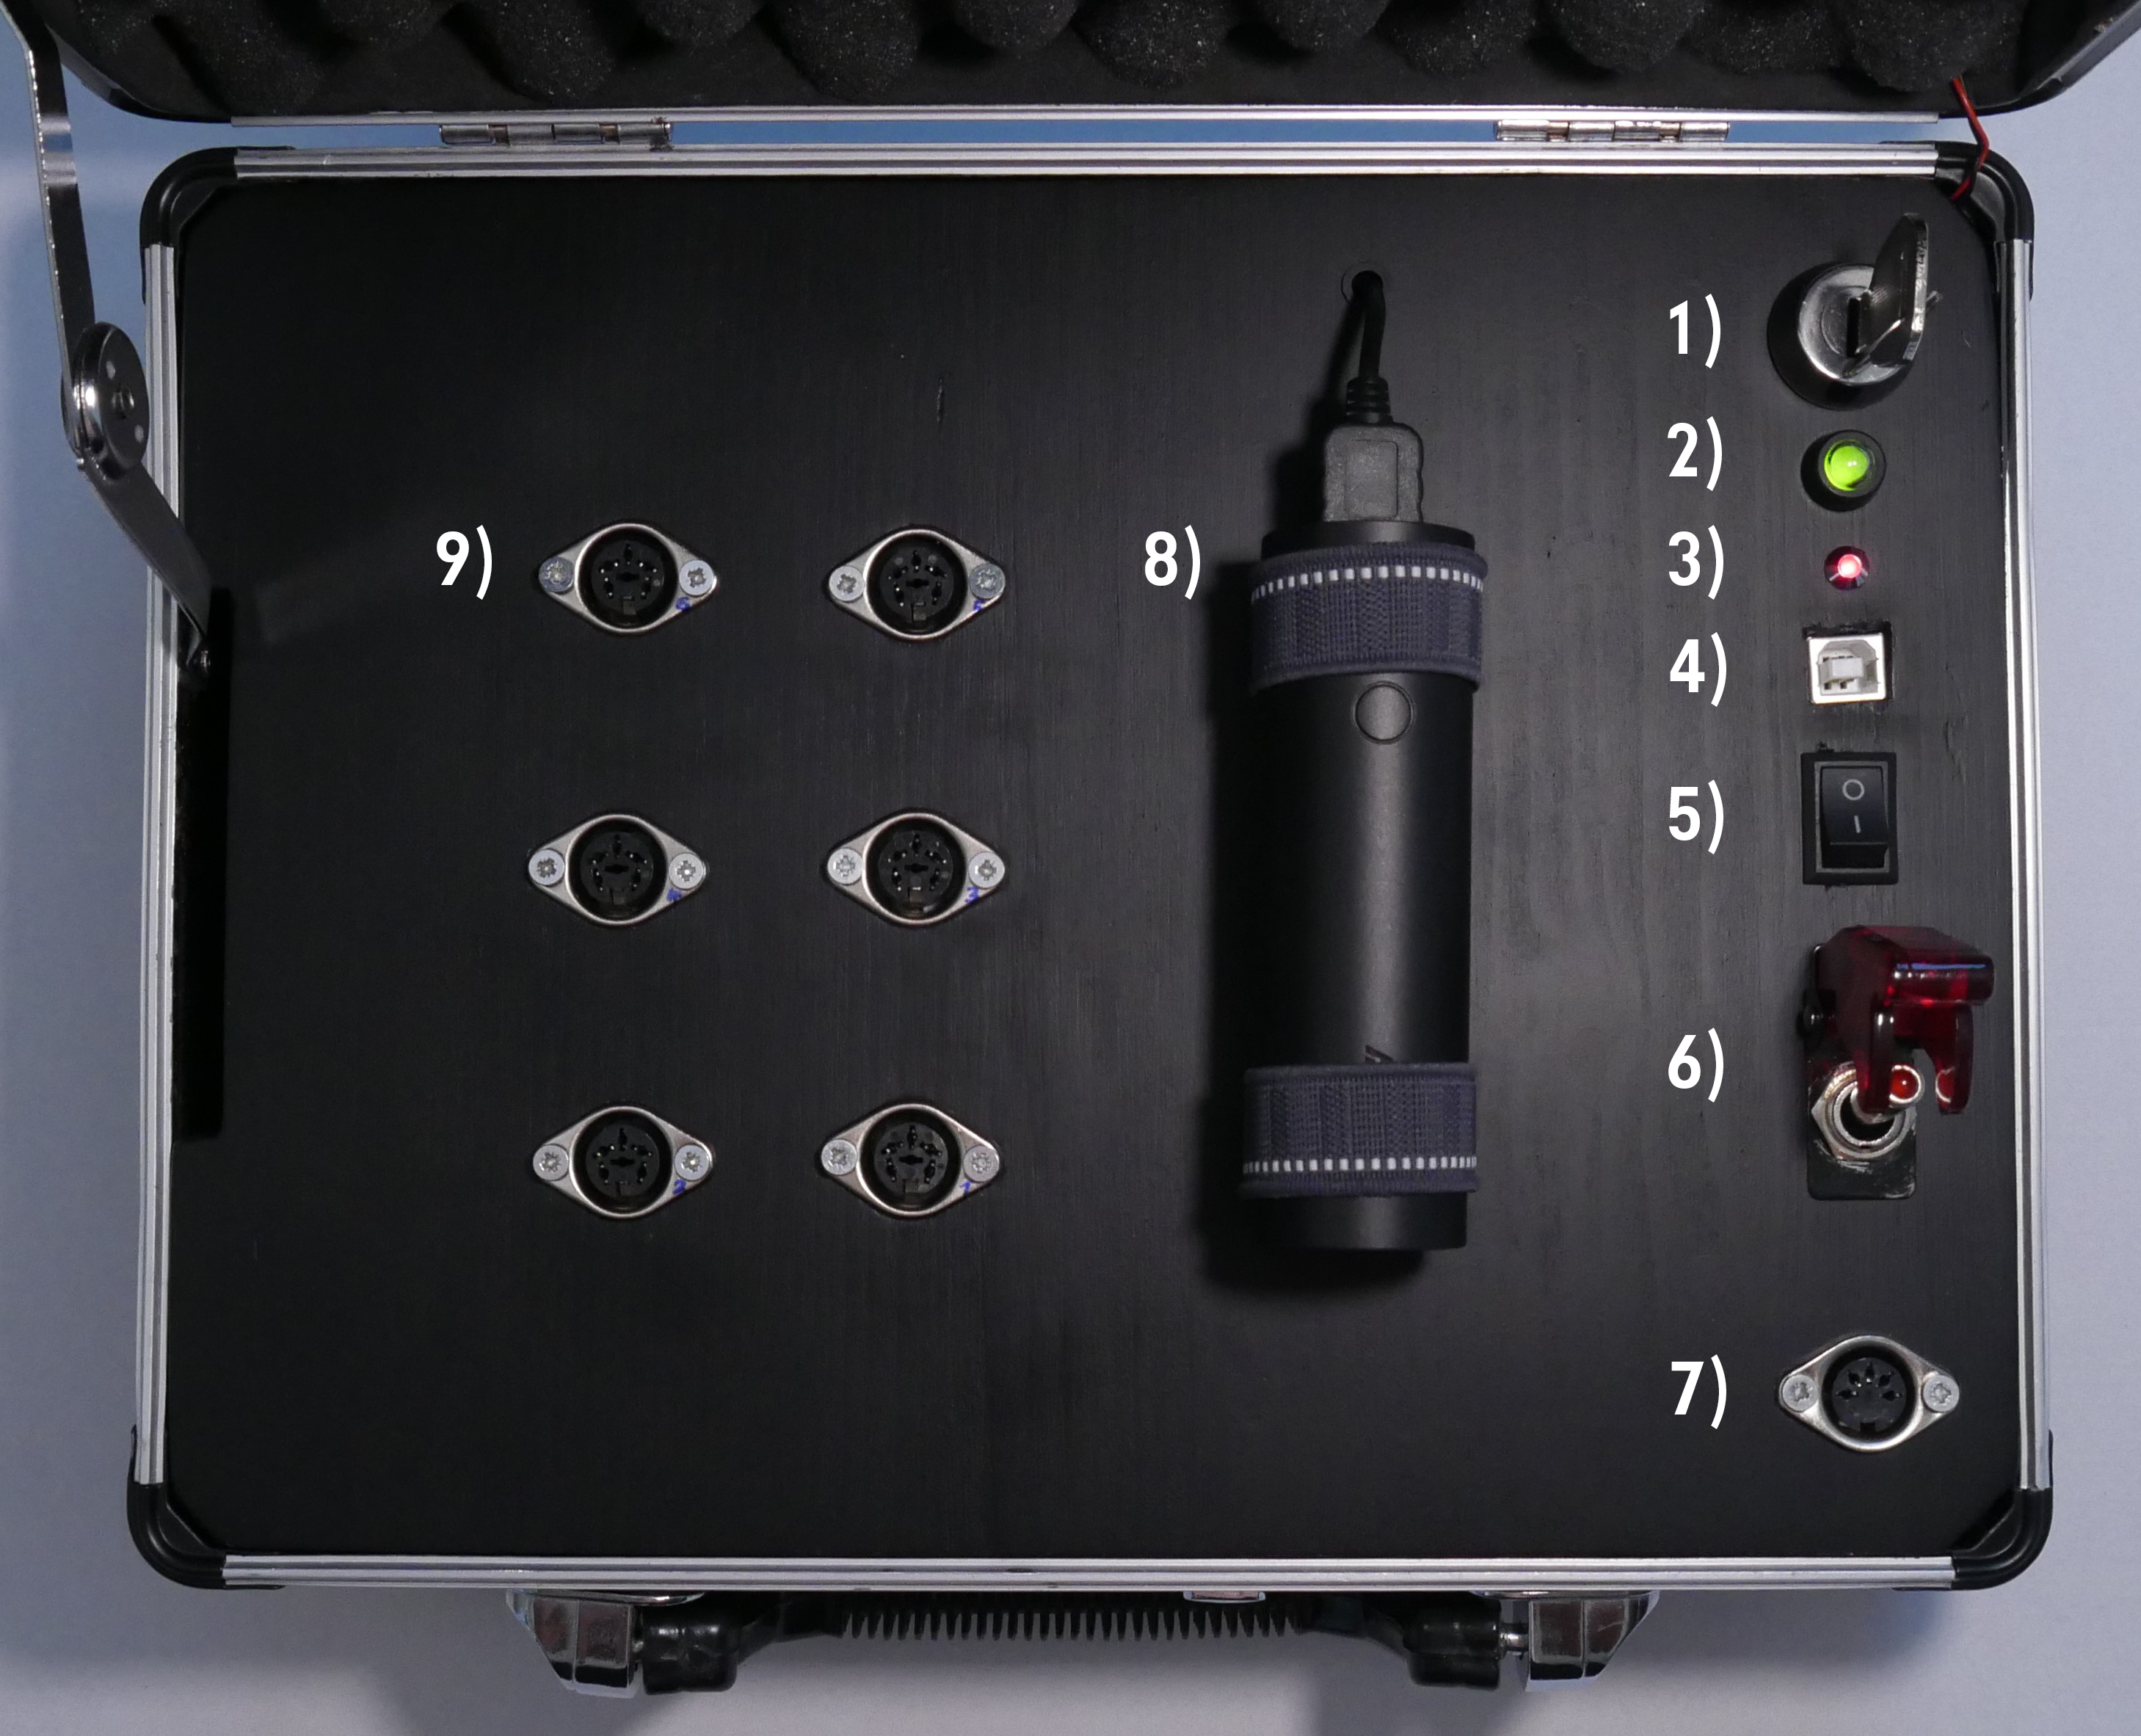
\includegraphics[width=10cm]{./Figures/controller_open_legend.png}
    \caption{ The complete controller and interface inside its case. }
    \label{fig:controller_open}     
\end{figure}

\begin{enumerate}
	\item ON/OFF key-switch
	\item Status LED 
	\item Ignition voltage reached indicator (See \Cref{Ignition Voltage Generator})
	\item USB female socket for programming
	\item Light ON/OFF switch
	\item Controller arm switch
	\item Trigger socket
	\item Power bank
	\item Module sockets
\end{enumerate}

\pagebreak

\subsection{Trigger}

\begin{figure}[!ht]
    \centering
    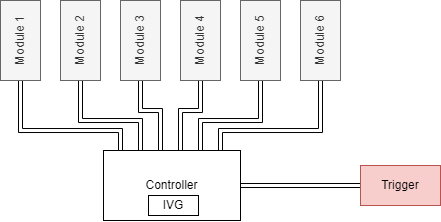
\includegraphics[width=5cm]{./Figures/concept_trigger.png} 
\end{figure}

\noindent The external trigger is responsible for setting off the pyrotechnic show. Its purpose is to tell the controller when to start but also tell the user that the state the controller is currently in. This is very important because the user must be far way from the controller when the pyrotechnics are ignited, but also needs to be informed if the system is working properly.

\subsubsection{Circuit}

\begin{figure}[!ht]
    \centering
    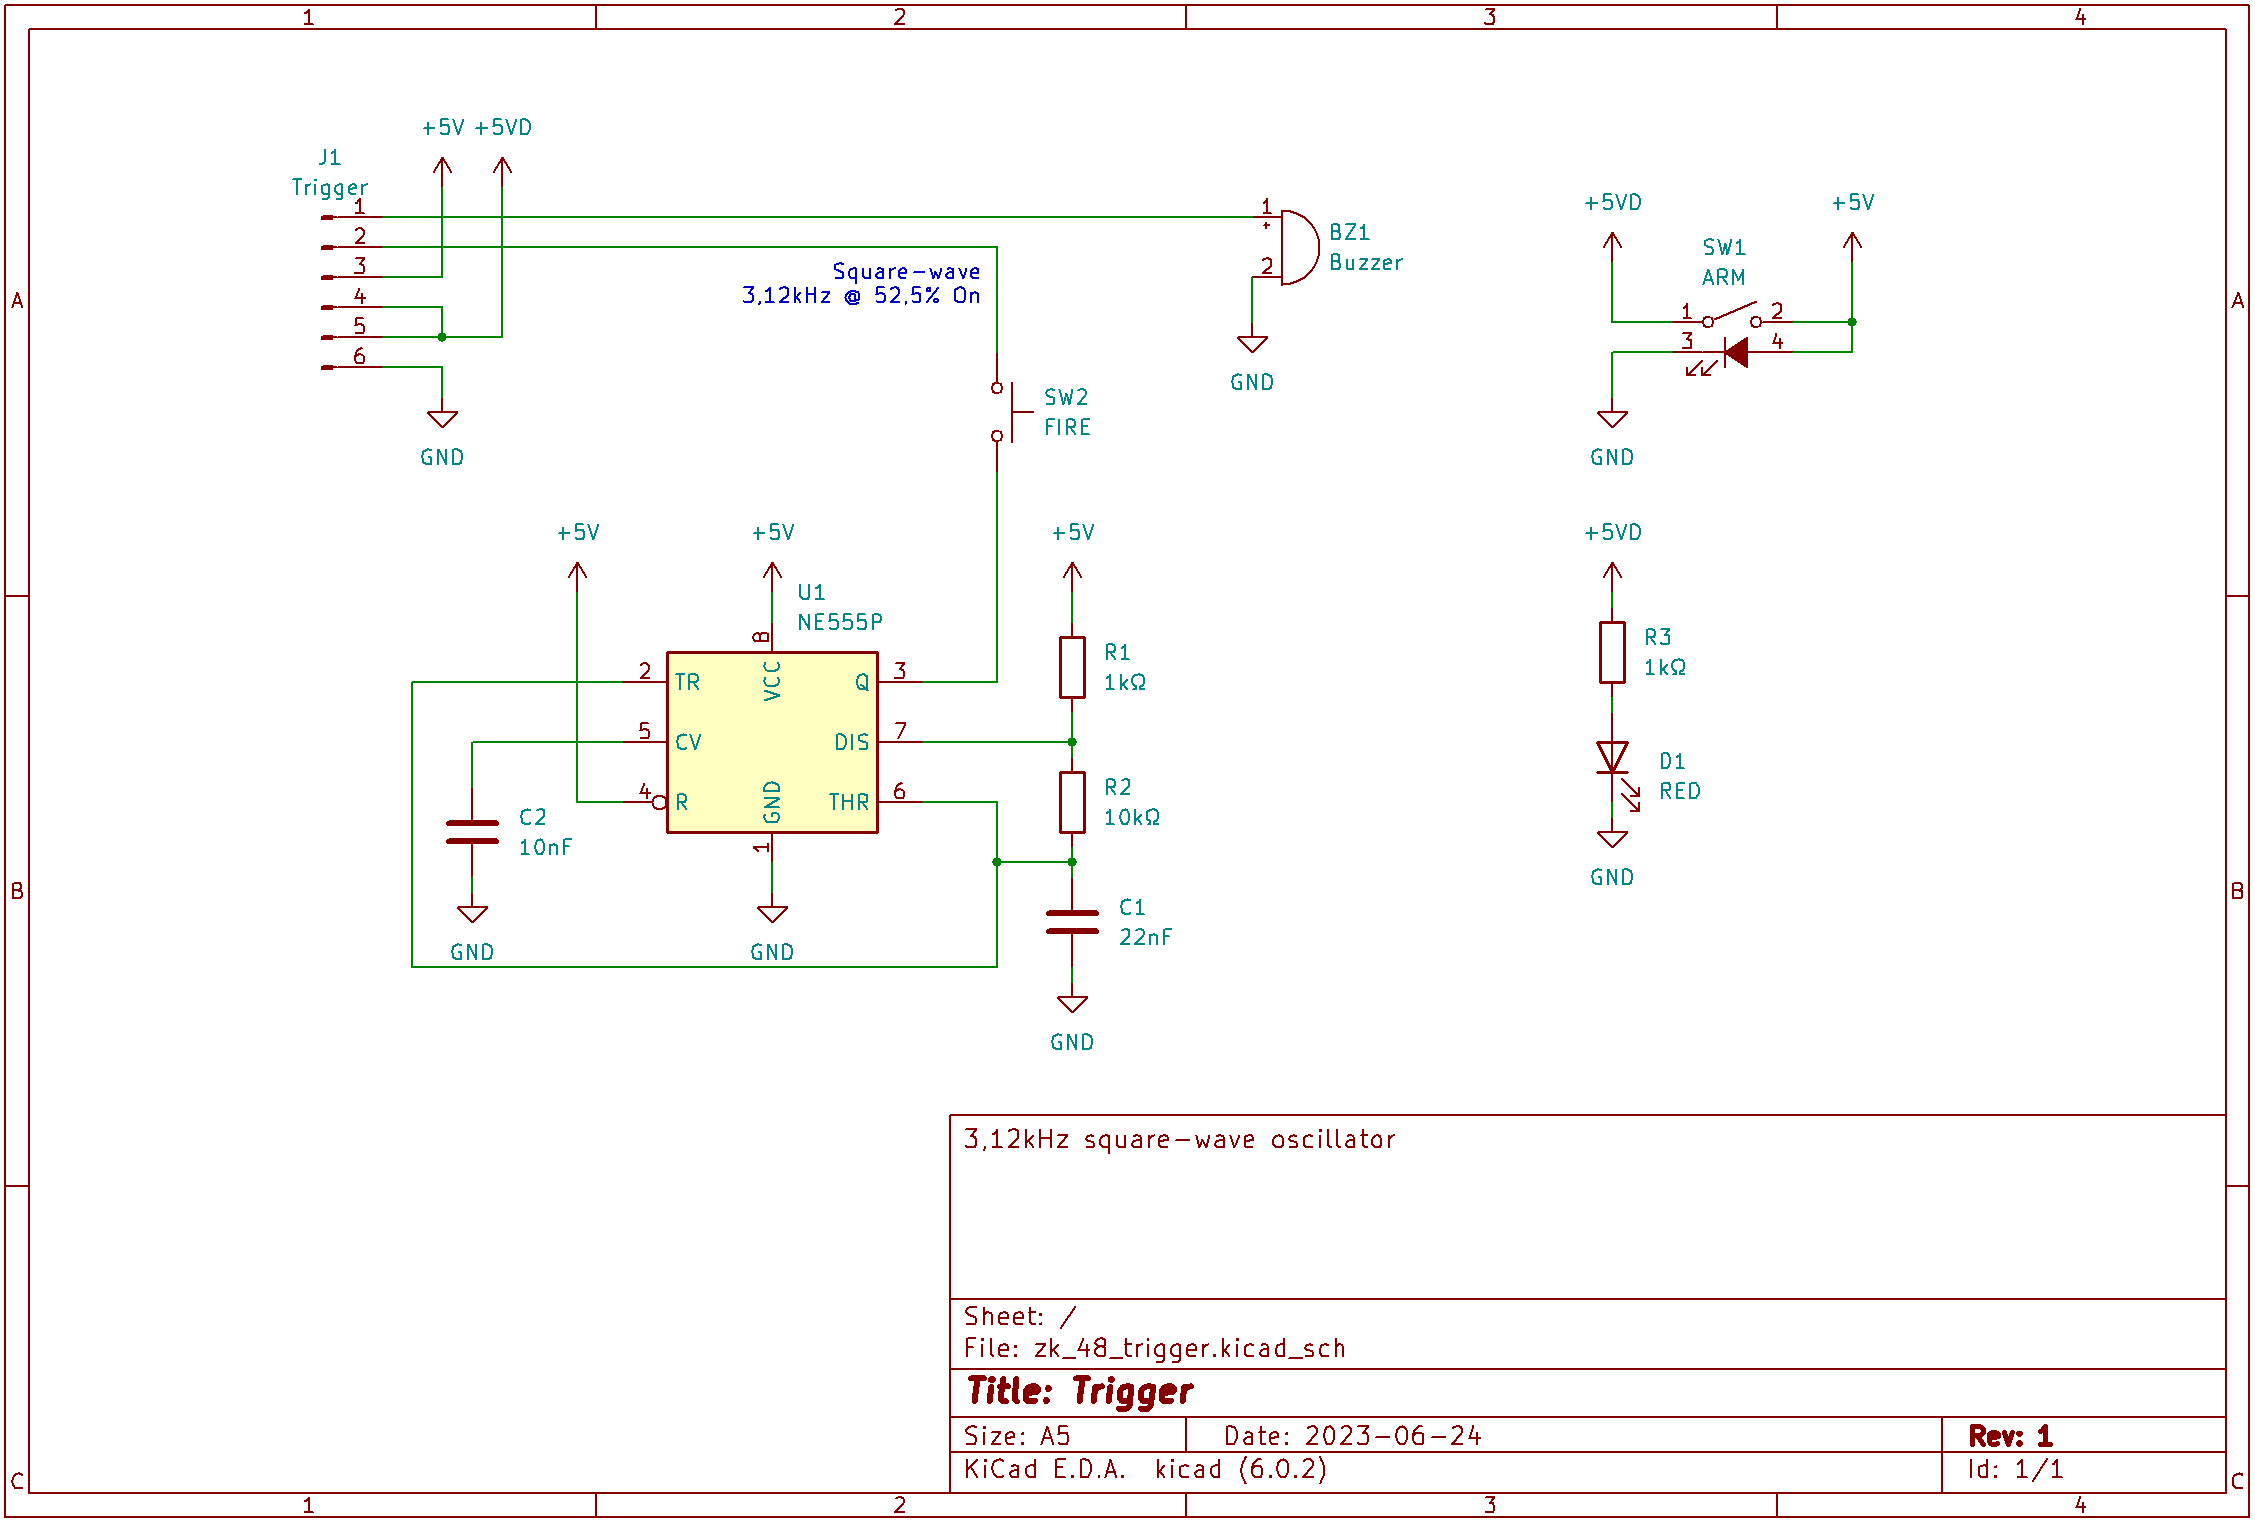
\includegraphics[width=15cm]{./Figures/trigger_circuit.png}
    \caption{The circuit of the external trigger.}
    \label{fig:trigger_circuit}     
\end{figure}

\pagebreak

\subsubsection{How does the trigger work?}
The trigger receives one signal and sends three signals back. The first 
input signal is going to buzzer and is connected to the buzzer on board the controller (See \Cref{fig:controller_circuit}). This buzzer gives the user feedback on the state of the system by changing the frequency of the sound produced by the buzzer. But more about this topic in \Cref{Firmware}. One of the three outputs is the CONCD signal, which stands for "Connected" and tells the µC if the trigger is plugged in. This output is straight connected to the $+5V$ power line.
The second output is the ARMED signal which indicates to the µC if the trigger is armed. This signal is produced by toggling the arm switch $SW1$ which also powers up the NE555 oscillator. If the trigger is armed, the NE555 will generate a $3,12kHz$ square-wave signal with a $52,2\%$ on-time. This signal is not passed through until the user holds down the fire $SW2$ button. Then the square-wave signal will be placed onto the FIRE line of the trigger, therefore starting the firing sequence. To indicate if the trigger has power, a small LED $D1$ is also present on the trigger.

\subsubsection{Housing}

\begin{figure}[!ht]
    \centering
    \includegraphics[width=10cm]{./Figures/trig_open.JPG}
    \caption{The external trigger circuit mounted inside its case.}
    \label{fig:trig_open}     
\end{figure}

\noindent The circuit of the trigger shown in \Cref{fig:controller_circuit} was soldered onto a perfboard. Together with the circuit, the arm switch, power LED and fire button were mounted into a ABS housing with the dimensions of 150x45x55mm as shown in \Cref{fig:trig_open}. The trigger uses a telephone cable, as described in \Cref{Housing of the Controller}, with a length of about $15m$ to connect to the controller. In \Cref{fig:trig_with_cable} the complete controller is visible.

\begin{figure}[!ht]
    \centering
    \includegraphics[width=10cm]{./Figures/trig_with_cable_legend.png}
    \caption{The external trigger with its cable.}
    \label{fig:trig_with_cable_legend}     
\end{figure}

\begin{enumerate}
	\item Arm switch
	\item Power LED
	\item Fire button
\end{enumerate}

\pagebreak

\subsection{Ignition Modules}
\label{Ignition Modules}

\begin{figure}[!ht]
    \centering
    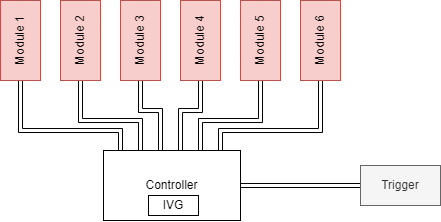
\includegraphics[width=5cm]{./Figures/concept_modules.png} 
\end{figure}

\noindent The ignition modules are responsible for the ignition of the pyrotechnic effects, therefore carry a large responsibility. There is no room for error and a 100\% success rate is required. Each module has eight ports for the bridge wire detonators to be connected.

\subsubsection{Circuit}

\begin{figure}[!ht]
    \centering
    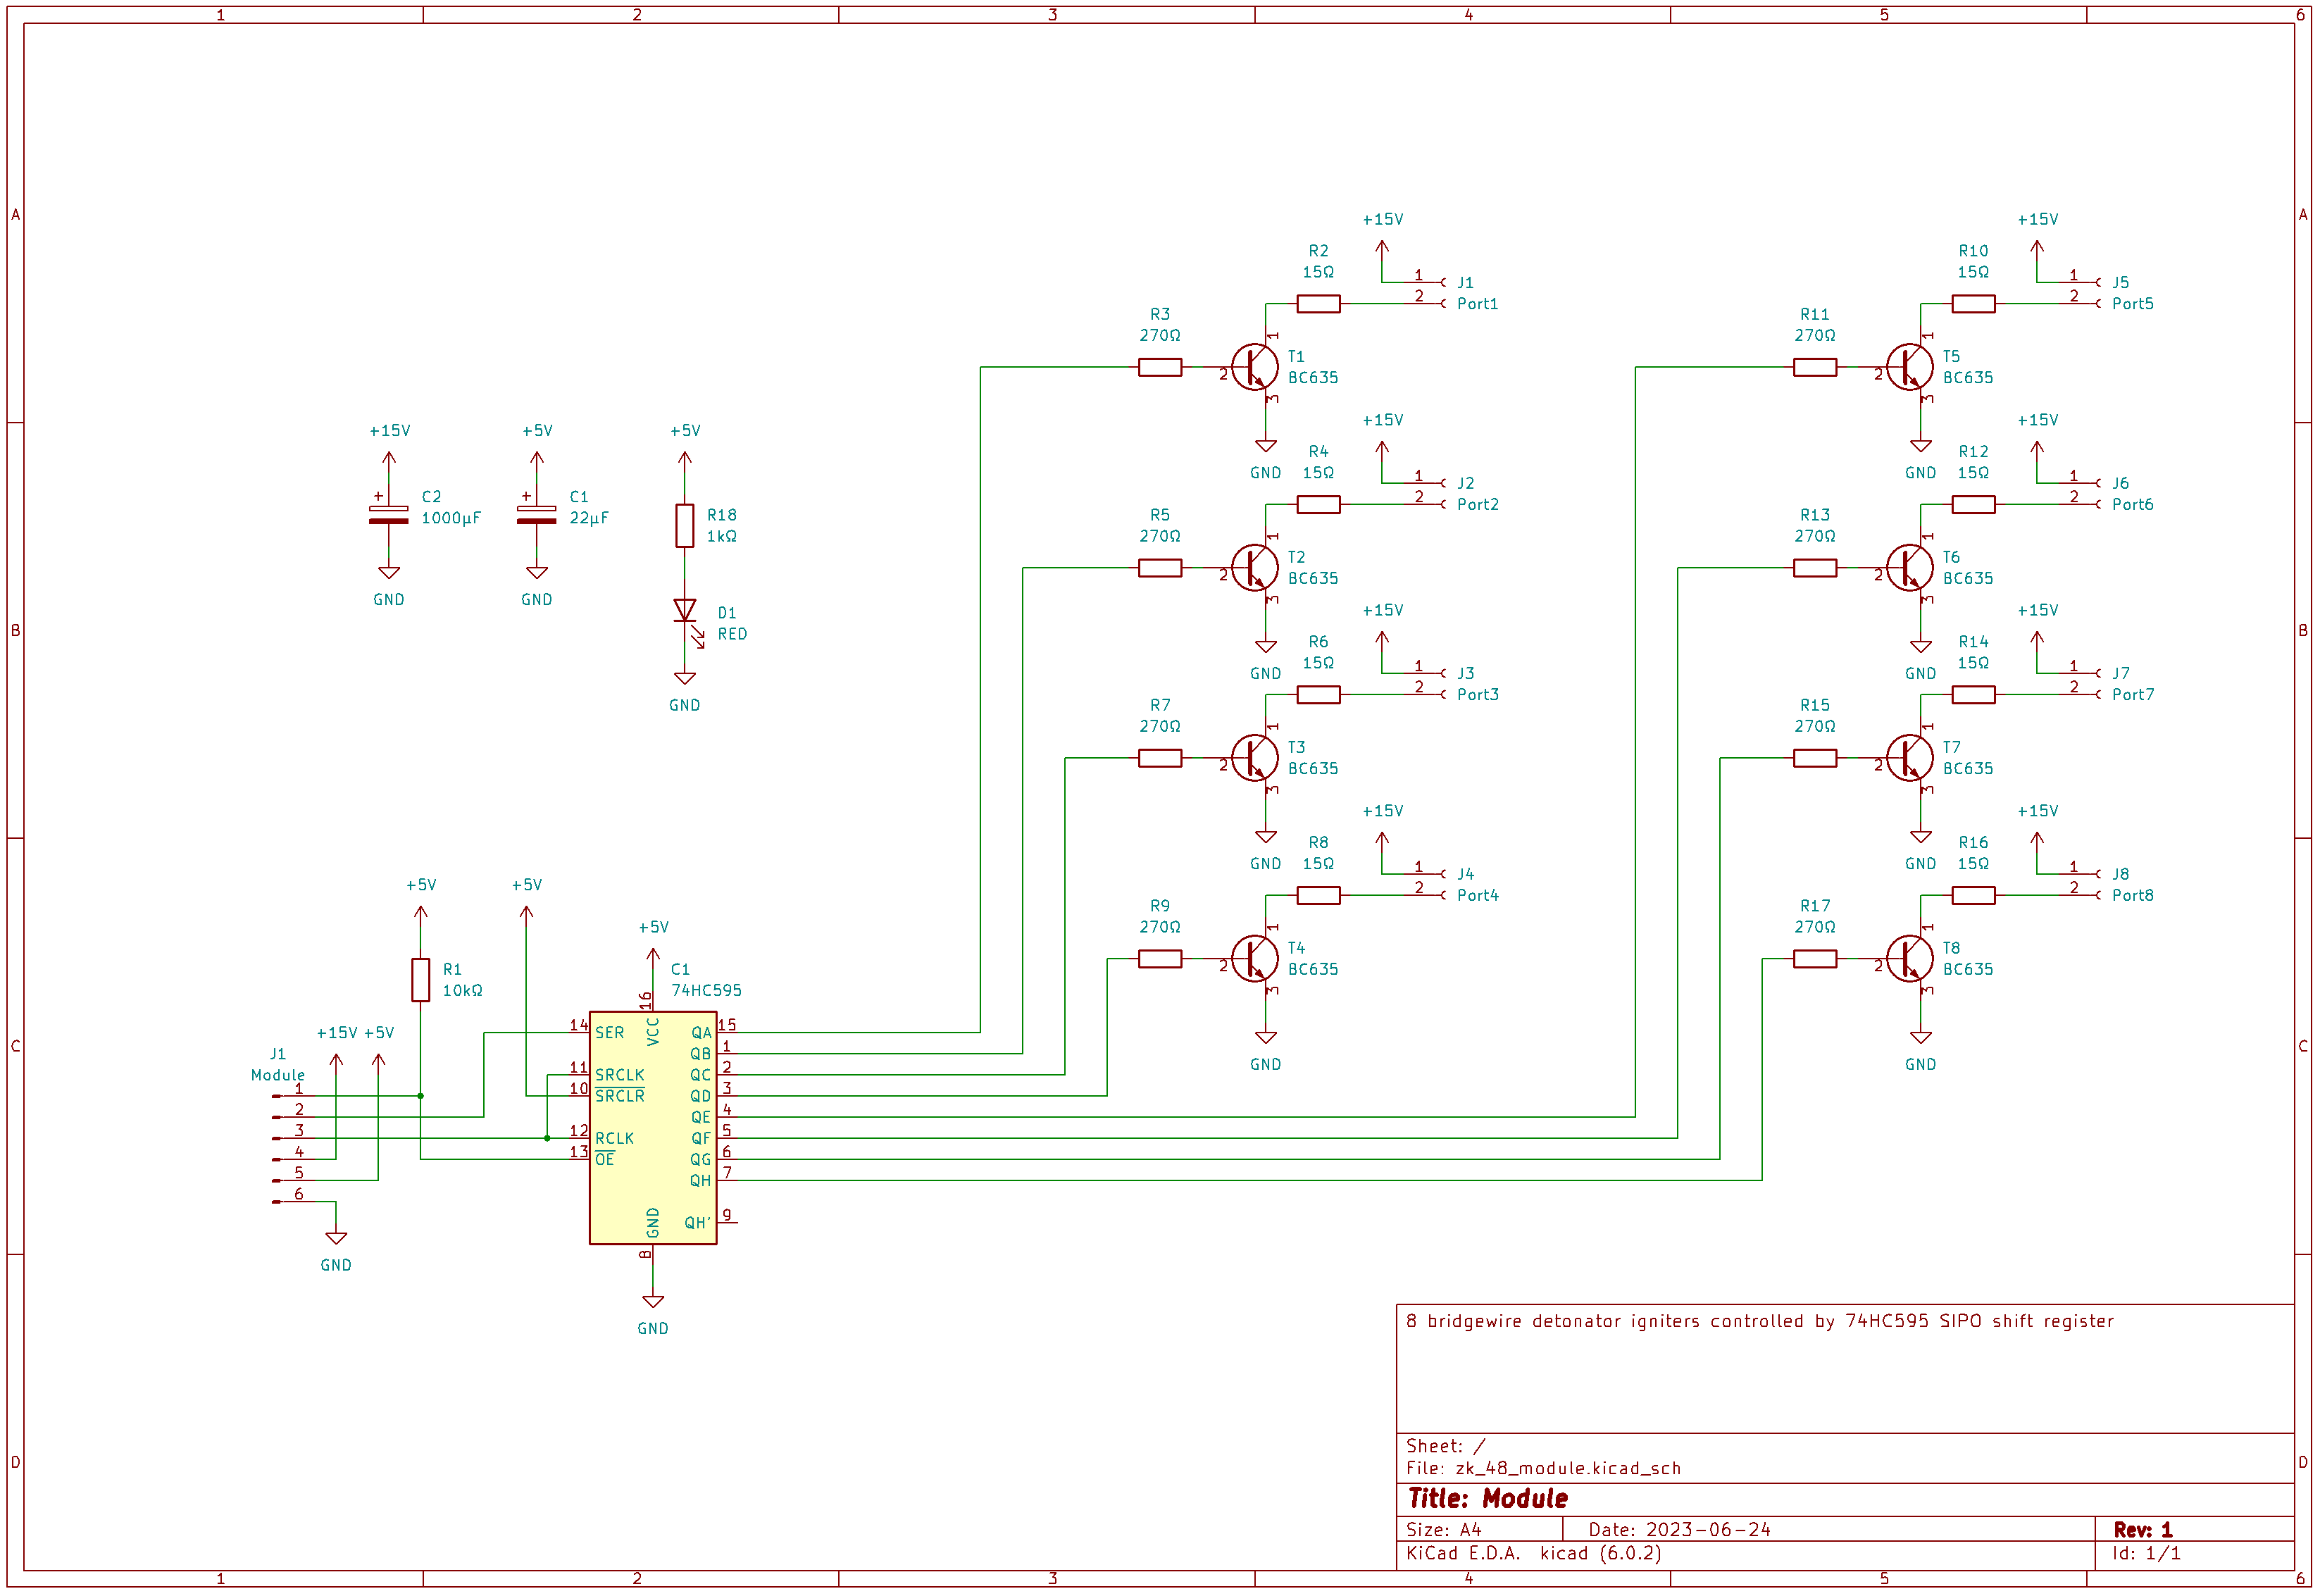
\includegraphics[width=15cm]{./Figures/module_circuit.png}
    \caption{The circuit of the ignition module.}
    \label{fig:trigger_circuit}     
\end{figure}

\pagebreak

\subsubsection{Housing}


\section{Firmware}
\label{Firmware}

\subsubsection{USB Connection}
\label{USB Connection}


\section{Software}
\label{Software}

\pagebreak

\section{Recognitions}
\label{Recognitions}
All circuits were drawn with the help of $KiCad\ 6.0$\footnote{\url{https://www.kicad.org/}}\\

\noindent All flowcharts and diagrams were drawn with the help of $Drawio$\footnote{\url{https://app.diagrams.net/}}



\end{document}
